% Format teze zasnovan je na paketu memoir
% http://tug.ctan.org/macros/latex/contrib/memoir/memman.pdf ili
% http://texdoc.net/texmf-dist/doc/latex/memoir/memman.pdf
% 
% Prilikom zadavanja klase memoir, navedenim opcijama se podešava 
% veličina slova (12pt) i jednostrano štampanje (oneside).
% Ove parametre možete menjati samo ako pravite nezvanične verzije
% mastera za privatnu upotrebu (na primer, u b5 varijanti ima smisla 
% smanjiti 
\documentclass[12pt,oneside]{memoir} 

% Paket koji definiše sve specifičnosti master rada Matematičkog fakulteta
\usepackage[latinica,biblatex]{matfmaster} 
\usepackage{listings}
\usepackage{verbatim}
%
% Podrazumevano pismo je ćirilica.
%   Ako koristite pdflatex, a ne xetex, sav latinički tekst na srpskom jeziku
%   treba biti okružen sa \lat{...} ili \begin{latinica}...\end{latinica}.
%
% Opicija [latinica]:
%   ako želite da pišete latiniciom, dodajte opciju "latinica" tj.
%   prethodni paket uključite pomoću: \usepackage[latinica]{matfmaster}.
%   Ako koristite pdflatex, a ne xetex, sav ćirilički tekst treba biti
%   okružen sa \cir{...} ili \begin{cirilica}...\end{cirilica}.
%
% Opcija [biblatex]:
%   ako želite da koristite reference na više jezika i umesto paketa
%   bibtex da koristite BibLaTeX/Biber, dodajte opciju "biblatex" tj.
%   prethodni paket uključite pomoću: \usepackage[biblatex]{matfmaster}
%
% Opcija [b5paper]:
%   ako želite da napravite verziju teze u manjem (b5) formatu, navedite
%   opciju "b5paper", tj. prethodni paket uključite pomoću: 
%   \usepackage[b5paper]{matfmaster}. Tada ima smisla razmisliti o promeni
%   veličine slova (izmenom opcije 12pt na 11pt u \documentclass{memoir}).
%
% Naravno, opcije je moguće kombinovati.
% Npr. \usepackage[b5paper,biblatex]{matfmaster}

% Pomoćni paket koji generiše nasumičan tekst u kojem se javljaju sva slova
% azbuke (nema potrebe koristiti ovo u pravim disertacijama)
\usepackage[latinica]{pangrami}

\usepackage{listings}
\usepackage{protobuf/lang}  % include language definition for protobuf
\usepackage{protobuf/style} % include custom style for proto declarations.


% Datoteka sa literaturom u BibTex tj. BibLaTeX/Biber formatu
\bib{literatura}

% Ime kandidata na srpskom jeziku (u odabranom pismu)
\autor{Ozren Demonja}
% Naslov teze na srpskom jeziku (u odabranom pismu)
\naslov{Realizacija P2P protokola za dostavu sinhronizovanog sadržaja}
% Godina u kojoj je teza predana komisiji
\godina{2018}
% Ime i afilijacija mentora (u odabranom pismu)
\mentor{dr Aleksandar \textsc{Kartelj}, docent\\ Univerzitet u Beogradu, Matematički fakultet}
% Ime i afilijacija prvog člana komisije (u odabranom pismu)
\komisijaA{dr Saša \textsc{Malkov}, profesor\\  Univerzitet u Beogradu, Matematički fakultet}
% Ime i afilijacija drugog člana komisije (u odabranom pismu)
\komisijaB{dr Miroslav \textsc{Marić}, profesor \\ Univerzitet u Beogradu, Matematički fakultet}
% Datum odbrane (odkomentarisati narednu liniju i upisati datum odbrane ako je poznat)
% \datumodbrane{}

% Apstrakt na srpskom jeziku (u odabranom pismu)
\apstr{%
}

% Ključne reči na srpskom jeziku (u odabranom pismu)
\kljucnereci{P2P mreža, deljenje video sadržaja, sinhronizovano deljenje sadržaja, P2P protokol, deljenje u realnom vremenu, decentralizovana razmena podataka}

\begin{document}
% ==============================================================================
% Uvodni deo teze
\frontmatter
% ==============================================================================
% Naslovna strana
\naslovna
% Strana sa podacima o mentoru i članovima komisije
\komisija
% Strana sa posvetom (u odabranom pismu)
\posveta{Mami i tati}
% Strana sa podacima o disertaciji na srpskom jeziku
\apstrakt
% Sadržaj teze
\tableofcontents*

% ==============================================================================
% Glavni deo teze
\mainmatter
% ==============================================================================

% ------------------------------------------------------------------------------
\chapter{Uvod}
% ------------------------------------------------------------------------------
\chapter{P2P mreža}
\label{chp:p2p-uvod}

Osnovna svrha interneta kao globalne mreže u današnje vreme je razmena digitalnog sadržaja. Arhitektura koja se koristi za podršku razmeni često je zasnovana na modelu klijent-server (eng. \textit{Client-Server architecture}). Model klijent-server deli zadatke između servera koji obezbeđuju resurse ili usluge i klijenata koji zahtevaju usluge \cite{DeBoever07}.

Kako svaki pristup sistemu od strane klijenta zahteva veću upotrebu resursa i bolje performanse, jasno se uočava da je server usko grlo sistema. 
Tokom 1990-ih godina internet se najvećim delom zasnivao na klijent-server modelu. Poslednjih desetak godina dolazi do velikog proboja novih tehnologija usled želje korisnika za interaktivnijim sadržajem, porastom brzine pristupa internetu (eng. \textit{broadband}), rasprostranjenosti pristupa, boljom stabilnosti veze i jačim računarima korisnika.

Navedene činjenice dovode do promene načina korišćenja interneta i pravljenja mreže ravnopravnih članova (eng. \textit{peer-to-peer (P2P) network}) u kojoj korisnici dele svoje resurse \cite{Tanenbaum}. Primena ovakvog pristupa obećavajuće je rešenje za mnoge oblasti.

U poglavlju \ref{P2P.1} opisani su osnovni koncepti mreže ravnopravnih članova. U poglavlju \ref{P2P.2} opisane su struktuirane i nestruktuirane mreže ravnopravnih članova. U poglavlju \ref{P2P.3} opisane su topologija stabla (eng. \textit{tree topology}), mrežna (eng. \textit{mesh topology}) i hibridna (eng. \textit{hybrid topology}) topologija. Način pripreme i slanja video sadržaja opisan je u poglavlju \ref{P2P.4}. U poglavlju \ref{P2P.5} opisani su osnovni problemi prilikom pravljenja mreže ravnopravnih članova.


\section{Osnovni koncepti}
\label{P2P.1}
Korišćenje aplikativnog sloja u formiranju pokrivača (eng. \textit{overlays}) za pristup internet servisima ima dugu istoriju. I pored duge tradicije ovakav pristup se do nedavno koristio samo za dizajn specifičnih protokola i interno povezivanje servisa infrastrukture, bez mogućnosti korišćenja između dva računara koja nisu susedi. Popularizacija ideje za formiranje pokrivača na aplikativnom sloju počinje 1999. godine sa Napster-om \cite{Aberer_2004} i nastavlja se kroz druge sisteme za razmenu digitalnog sadržaja kao što su Gnutella \cite{Gnutella}, FastTrack \cite{FastTrack}, KaZaa \cite{kazaa} i BitTorrent \cite{Bittorent}. 

Arhitektura ravnopravnih članova (eng. \textit{peer-to-peer, P2P}) definiše se kao distribuirani vid arhitekture u kojoj svaki parnjak (eng. \textit{peer}) može samostalno da obavlja poslove, ali omogućava drugim parnjacima da koriste njegove resurse kao što i sam može po potrebi koristiti resurse drugih parnjaka \cite{Shen:2009}. Drugim rečima, svaki parnjak komunicira sa ostalim parnjacima u mreži koristeći softver koji se ponaša i kao klijent i kao server. Na osnovu navedenih činjenica zaključuje se da arhitektura ravnopravnih članova omogućava veću autonomiju članova mreže koji sami definišu pravila o deljenju resursa. Glavna primena arhitekture ravnopravnih članova prisutna je u sistemima sa većom tolerancijom greške kod distribuirane obrade. Pored toga, ovaj vid arhitekture koristi se prilikom razmene fajlova, direktne komunikacije, obrade velikih količina podataka i softvera za zabavu. 


Prilikom deljenja resursa svaki parnjak doprinosi resursima mreže ravnopravnih članova. Idealno, deljenje resursa je proporcionalno broju parnjaka koji koriste mrežu ravnopravnih članova. Međutim, usled različitih problema u praksi navedeno svojstvo većinom nije ispunjeno. 

P2P sistem čini skup međusobno povezanih parnjaka, direktno ili preko drugih parnjaka formirajući povezani graf. Kako u grafu ne postoji centralna tačka kontrole i kolektivno se obavlja posao, P2P sistemi su decentralizovani. U nekim situacijama definiše se centralni server za poslove kao što su identifikacija, autentikacija i različite sigurnosne provere. U ovakvim uslovima, po pravilu server obavlja što je moguće manji deo posla. Pored toga, ponekad se u P2P sistemima iz različitih razloga uvode parnjaci zaduženi za dodatni deo posla.
Ovakvi parnjaci se nazivaju super parnjaci (eng. \textit{super peers}).


Učešće parnjaka u obavljanju posla u P2P sistemima određeno je lokalno. Iz ove činjenice proizilazi bolja organizacija P2P sistema vremenom usled korišćenja lokalnih znanja i operacija na svakom parnjaku. Ovim se takođe sprečava neplanirana dominacija nekog parnjaka sistemom.

Dva važna svojstva P2P sistema su samoskalabilnost i stabilnost. 
Samoskalabilnost, kao glavna prednost P2P sistema,
ispoljava se povećanjem ukupne snage sistema prilikom pristupanja parnjaka. Stabilnost mreže se obično definiše kao njena otpornost na veliku stopu promene strukture mreže usled čestog dolaska i odlaska parnjaka. U literaturi ove promene se nazivaju talasanja (eng. \textit{churn}). P2P sistem bi trebao biti stabilan do određenog nivoa talasanja, u kontekstu održavanja grafa konekcije i upućivanja (eng. \textit{route}) sadržaja deterministički sa prihvatljivim granicama broja skokova (eng. \textit{hop-count bounds}).


P2P sistem, kao tehnologija u zamahu, privlači veliku pažnju običnih i korporativnih korisnika. Takođe, pored pažnje korisnika, značajno interesovanje beleži se i u istraživačkim krugovima \cite{DeBoever07}. U poslednjih nekoliko godina, veliki deo istraživanja bavi se P2P deljenjem resursa i prenosom podataka. 

\section{Klasifikacija P2P mreža}
\label{P2P.2}

Usled velikog broja kriterijuma dizajniranja P2P mreža, ne postoji jedinstven način klasifikacije \cite{Shen:2009}. Na primer, sistemi za deljenje fajlova često se klasifikuju po generacijama. Prvu generaciju karakteriše hibridni dizajn. Glavnu karakteristiku ove generacije predstavlja kombinacija servera sa P2P upućivanjem sadržaja. Druga generacija je zasnovana na decentralizovanoj arhitekturi. Trećom generacijom smatraju se anonimni P2P sistemi kao što su Freenet \cite{Clarke_2001} i I2P \cite{I2P}. Ovakav način kategorizacije prema generacijama ima značajnih nedostataka. Glavni nedostatak ogleda se u nedefinisanim važnim dimenzijama problema i nejasnoći dodatnih mogućnosti sledeće generacije. Takođe, sistemi sve tri generacije su korišćeni u isto vreme što se ne može zaključiti na osnovu njihovih imena. Zbog navedenih nedostataka, u literaturi se češće sreće podela prema P2P pokrivaču. Prema ovoj podeli, razlikujemo struktuiranu i nestruktuiranu P2P mrežu  \cite{Prasanna_Ganesan_2004}.

U struktuiranim P2P mrežama topologija je precizno definisana. 
Takođe, neophodna je striktna kontrola protoka sadržaja. Sadržaj se ne sme nalaziti kod proizvoljnih parnjaka već mora biti na strogo definisanim lokacijama koje će omogućiti efikasniju pretragu.
Većina struktuiranih P2P mreža je bazirana na distribuiranim heš tabelama (eng. \textit{Distributed Hash Table (DHT)}). Kao primere struktuiranih P2P mreža navodimo Tapestry \cite{Zhao_2004}, Chord \cite{Stoica_2003}, Pastry \cite{Rowstron_2001} i Kademlia \cite{Maymounkov_2002}.

Ne struktuirani P2P sistem je sačinjen od parnjaka koji se pridružuju mreži sa nekim labavim skupom pravila, bez ikakvog predznanja o njenoj topologiji. Freenet, Gnutella, FastTrack, KaZaA i BitTorrent su primeri ovakvih sistema. Ovakve mreže se zbog svojih svojstava tipično koriste za udruživanje snage parnjaka nebi li se neki posao brže obavio ili razmenu fajlova kod kojih nije od presudnog značaja brzina pronalaska fajla. 

U nestruktuiranim P2P mrežama, pretraga je bazirana na prosleđivanju upita. Svaki parnjak upit prosleđuje komšijama, osim u slučaju kada parnjak može odgovoriti na traženi upit ili se brojač skokova upita smanji na 0 \cite{Shen:2009}. Sa ovakvim načinom prosleđivanja postoje različita pravila kontrole prosleđivanja upita. Način prosleđivanja može se kontrolisati tako što se upit neće proslediti svim komšijama nego samo određenim. Izbor kome će upit biti prosleđen se vrši prema informacijama koje parnjak čuva o komšijama. Te informacije predstavljene su istorijom ili indeksima sadržaja koji komšija može obezbediti. Takođe, često se prosleđivanje vrši slučajno bez ikakvog znanja. Naravno, ovo svojstvo smanjuje šansu da se pronađe sadržaj. 
Opravdanje nestruktuiranog pristupa zasniva se na promenljivosti broja članova mreže i ispravnosti prvog izbora komšije.

Nestruktuirane mreže ravnopravnih računara uglavnom su sastavljene od parnjaka koji su kućni PC računari. Oni su najčešće povezani sa mrežom slabim propusnim opsegom (eng. \textit{bandwidth}). Takođe, većinom je propusni opseg nesrazmeran u odnosu na dolazni i odlazni saobraćaj u korist dolaznog saobraćaja. Navedena činjenica blago narušava samoskalabilnost mreže. Postoje različiti načini da se spreči narušavanje samoskalabilnosti. Neki od njih su zasnovani na kažnjavanju parnjaka koji ne doprinose ili jako malo doprinose resursima sistema. 


\section{Topologija}
\label{P2P.3}

P2P sistem je sačinjen od dva podsistema koji se izvršavaju paralelno. To su konstrukcija i održavanje izabrane topologije kao i prosleđivanje bloka (eng. \textit{chunk}) podataka. Algoritmi za konstrukciju i prosleđivanje zajedno formiraju P2P protokol. U zavisnosti od odluka donešenih pri dizajnu sistema tj. od izabrane topologije i algoritma prosleđivanja može se napraviti P2P sistem sa različitim karakteristikama.

\subsection{Topologija drveta}
\label{P2P.3.1}

Među prvim predloženim topologijama P2P sistema za razmenu sadržaja predstavljena je topologija drveta. U okviru ove topologije, svi parnjaci su organizovani tako da čine strukturu drveta. Primer topologije drveta prikazan je na slici \ref{fig:topologija-drveta}.
 
\begin{figure}[!ht]
  \centering
  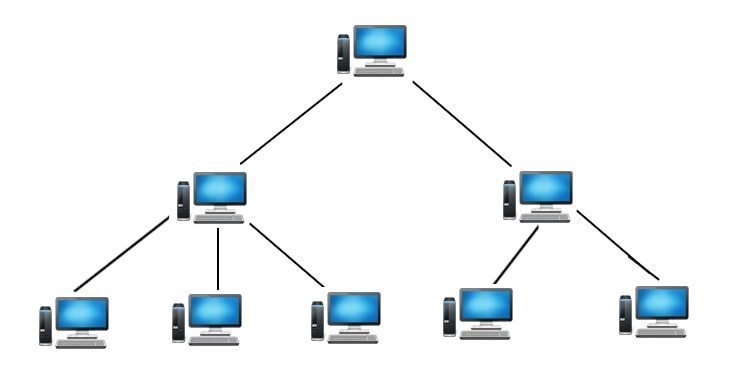
\includegraphics[width=1.05\textwidth]{slike/tree-topology.jpg}
  \caption{Primer topologije drveta}
  \label{fig:topologija-drveta}
\end{figure}
\par

U korenu drveta nalazi se parnjak koji deli sadržaj-izvor. Svaki parnjak u sistemu može imati tačno određeni broj dece koji je ili unapred definisan ili određen kapacitetom parnjaka. Deca su komšije koje preuzimaju sadržaj od roditelja. Konstrukcija drveta i relacija roditelj-dete može biti određena različitim faktorima kao što su ukupno vreme potrebno da podatak stigne od izvora do svih parnjaka u mreži, dostupan propusni opseg i fizička topologija same mreže. Podaci koji se šalju na ovakav način se najpre podele na manje delove koji se nazivaju paketi. Paket se zatim šalje od izvora do parnjaka koji se nalaze na prvom nivou drveta. Nakon toga parnjaci sa prvog nivoa drveta šalju podatke parnjacima na drugom nivou drveta i tako redom sve dok paket ne dođe do svih parnjaka u mreži \cite{DeBoever07}.

Iako jednostavna za konstrukciju, topologija drveta ima dosta nedostataka. Najveći nedostatak je neravnomerna raspodela tereta prosleđivanja koja se javlja kao posledica činjenice da veliki deo parnjaka čine listovi koji ne daju nikakav doprinos sistemu. Dodatno, parnjak koji nema odlazni (eng. \textit{upload}) kapacitet proporcionalan proizvodu broja dece i veličine bloka koji prenosi, konstantno će nagomilavati blokove podataka i usporavati ceo sistem. Ovakav parnjak treba da bude lociran jedino u listovima stabla ili veoma blizu listova. 
Pored navedenih osobina, važno je napomenuti da je ovakva struktura ranjiva na napuštanje parnjaka. Prilikom napuštanja parnjaka na višem nivou, njegova podstabla privremeno ostaju odsečena od ostatka mreže.

Da bi se povećala otpornost na napuštanja parnjaka i povećao kapacitet mreže koristi se rešenje bazirano na višestrukim stablima. U ovakvim sistemima parnjaci se nalaze u jednom ili više stabala. Svaki parnjak prima sadržaj od svih stabala čiji je član. Izvorni čvor je izvor za sva stabla. Dobijen sadržaj parnjak prosleđuje unapred određenim stablima. Sistem se na ovaj način deli u podsisteme u kojima svaki od podsistema predstavlja jedno stablo. Radi bržeg distribuiranja sadržaja svakom podsistemu se dodeljuje jedinstven paket.

Topologija zasnovana na višestrukim stablima rešava neke od problema upotrebe samo jednog stabla, ali uvodi dodatne probleme \cite{DeBoever07}. Prvo, na ovakav način postoji više putanja od izvora do lista pa je potreban značajno složeniji algoritam prosleđivanja. Drugo, kako stabla imaju različite podatke potrebno je obezbediti da svi podaci dođu do svakog parnjaka. Treće, prilikom konstrukcije mreže treba kreirati stabla koja su što je moguće manje dubine čime bi se obezbedio brži protok podataka. Dodatno, javlja se povremena potreba prebacivanja parnjaka iz jednog stabla u drugo uz dodatni zadatak balansiranja dubina svih stabala. Četvrti problem leži u balansiranju kapaciteta stabala. 

\subsection{Topologija mreže}
\label{P2P.3.2}

Sistem zasnovan na mreži se fokusira na kreiranje topologije koja se brzo adaptira na promene. Glavna ideja pri pravljenju ove topologije bila je da parnjaci provode što je moguće manje vremena za održavanje pokrivača i brzi oporavak mreže pri njihovom napuštanju. Prednost ove topologije je brža i jednostavnija konstrukcija pokrivača. Sa druge strane, u ovakvoj konstrukciji potrebno je uložiti značajno vreme za implementaciju algoritma za prosleđivanje sadržaja između parnjaka. Primer topologije mreže nalazi se na slici \ref{fig:topologija-mreze}.
 
\begin{figure}[!ht]
  \centering
  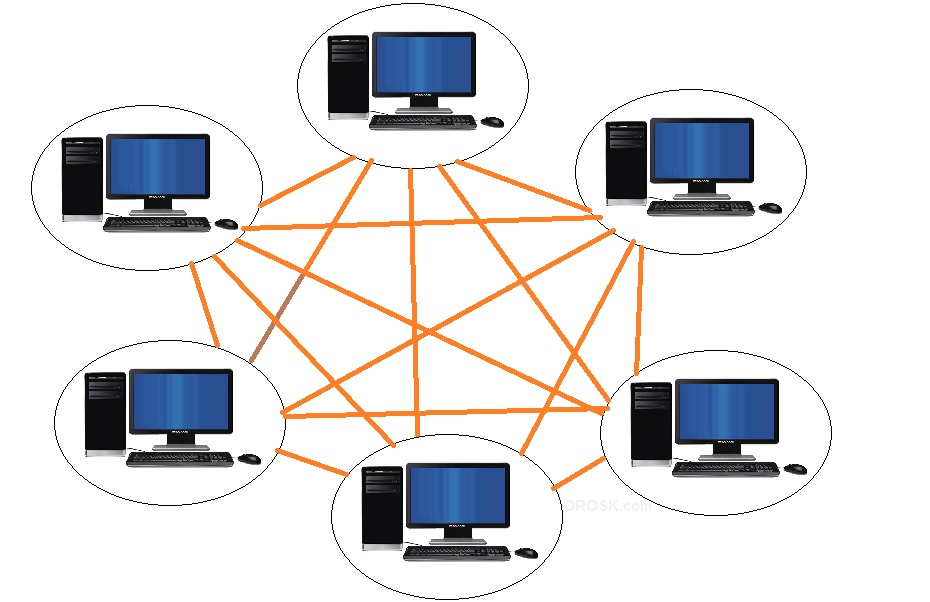
\includegraphics[width=1.05\textwidth]{slike/mesh-topology.jpg}
  \caption{Primer topologije mreže}
  \label{fig:topologija-mreze}
\end{figure}
\par

Značajan kontrast se može primetiti ukoliko se posmatraju razlike između topologije mreže i topologije drveta \ref{P2P.3.1}. Kod topologije drveta kreiranje same topologije je složenije i zahteva više vremena, ali jednom kad se postigne željeni dizajn mreže prosleđivanje podataka je jednostavno. Kod topologije mreže situacija je potpuno drugačija. Sama izrada pokrivača je krajnje jednostavna, jeftina i brza, ali je prosleđivanje podataka značajno kompleksnije. 

U mrežnom pokrivaču glavni cilj parnjaka je da održavaju veliki broj dolaznih konekcija \cite{Shen:2009}. U slučaju izlaska komšije iz mreže, njegov uticaj na parnjake je minimalan. Pokrivač se obično gradi na distribuirani način i svaki parnjak je svestan samo malog dela učesnika, njegovih komšija. Način biranja komšija se razlikuje od politike (eng. \textit{policy}) do politike,
pri čemu je u svim slučajevima ovaj proces brz i jednostavan. Primer brze i jednostavne politike je slučajno biranje komšija. 

U odnosu na topologiju drveta, prosleđivanje podataka u mreži ne odvija se pravolinijski. Nedostatak konkretne strukture koja bi definisala put kojim paket treba ići čini nemogućim određivanje unapred putanje kojom paket treba proći. Zbog navedenog svojstva prosleđivanje paketa je bazirano na lokalnim odlukama koje svaki parnjak donese. Parnjaci donose odluke prema informacijama koje imaju o komšijama. Paket se može razmeniti primenom guranja (eng. \textit{push}) ili povlačenja (eng. \textit{pull}). Kod guranja parnjak određuje koji paket šalje svakom komšiji, a kod povlačenja određuje koji paket traži od svakog komšije. Oba pristupa imaju dobre i loše strane. 

Pristup sa guranjem je efikasniji u mreži sa ograničenim odlaznim kapacitetom jer izbegava višestruke zahteve za pakete. Pristup sa povlačenjem je dobar izbor za mreže sa ograničenim dolaznim kapacitetom jer parnjak može da kontroliše koliko brzo će primati pakete od komšija. Kod obe šeme zbog lokalne koordinacije propagacije paketa dolazi do blage neefikasnosti u prosleđivanju. Kod sistema guranja ova činjenica se ogleda u višestrukim kopijama koje parnjak može da dobije ako mu više komšija šalje isti paket. Kod sistema povlačenja može se desiti da komšije zaguše parnjaka sa previše zahteva za paketima. Takođe sistemi povlačenja unose dodatan sadržaj u mrežu (eng. \textit{overhead}) s obzirom da se paket mora tražiti.

\subsection{Hibridna topologija}
\label{P2P.3.3}

Hibridna topologija kombinuje prednosti topologija drveta i mreže. Preciznije, predstavlja kombinaciju robusnosti mrežne topologije sa jednostavnošću i efikasnošću prosleđivanja paketa koju nudi topologija drveta.

U hibridnoj topologiji, mreža je podeljena na više podmreža slično kao kod topologije drveta \cite{Shen:2009}. Da bi parnjak mogao da prima pakete, mora pronaći roditelje koji će mu prosleđivati pakete iz svih podmreža. Kada se novi parnjak pridružuje mreži, on dobija listu svih parnjaka na koje može da se poveže. Zatim parnjak među njima pokušava da odabere komšije tako da pokrije sve podmreže. Nakon što je pronašao takve parnjake povezuje se na njih. Glavna mana ovakvog sistema je ta što je dobijanje pravilne topologije težak zadatak. Često se može desiti da mala greška dovodi do situacije da parnjak ili grupa parnjaka bude izolovana od ostatka mreže.

\section{Protok video sadržaja}
\label{P2P.4}

Od samog nastanka, video je važan mediji za komunikaciju i zabavu. Sačinjen je od serije slika koje se smenjuju odgovarajućom brzinom dajući privid neprekidnog kretanja. Ovaj trik bio je poznat još u drugom veku u Kini, ali je ostao nepoznat ostatku sveta sve do 19. veka. Otkrićem kamere 1888. godine omogućeno je "automatsko" hvatanje i čuvanje pojedinačnih komponenti slike na filmskoj traci. Emitovanje televizijskog signala, nakon izuma 1928. godine, omogućilo je bilionima ljudi širom sveta uživo praćenje snimljenog sadržaja. Zahvaljujući širokoj dostupnosti signala, primarni vid zabave i dobijanja informacija umesto novina i radija postala je televizija.

Tokom većeg dela 20. veka, jedini način dobijanja televizijskog signala bio je preko vazduha ili kabla. Ranih 2000-tih internet doživljava veliki rast propusnog opsega. Pored rasta propusnog opsega svakodnevno se razvijaju bolji algoritmi kompresije video snimaka čime se omogućava da se sa značajno manje podataka predstavi isti snimak bez velikih gubitaka na kvalitetu.
Takođe, značajnu ulogu u svemu igra i Murov zakon \cite{Moore} činjenicom da eksponencijalni porast snage računara omogućava rešavanje raznovrsnijih problema. Navedena svojstva omogućavaju da sistem za dostavu video sadržaja u realnom vremenu (eng. \textit{streaming}) putem interneta postane moguć. Dostava video sadržaja u realnom vremenu omogućava emitovanje pre preuzimanja celokupnog sadržaja. Video se neprekidno šalje i emitovanje se omogućava odmah po pristizanju ili sa određenom zadrškom \cite{Telecom}.

Internet je dizajniran za slanje paketa bez mogućnosti kontrole toka. Ovakav način transfera ne pogoduje slanju vremenski neprekidno baziranog saobraćaja kao što su video i audio sadržaji \cite{Tanenbaum}. Glavni razlog je što dostava u realnom vremenu ima određeni poredak kojim se mora emitovati kao i vremenska ograničenja. Na primer, video sadržaj se mora emitovati neprekidno slika za slikom. U slučaju da podatak ne stigne na vreme, proces emitovanja će biti prekinut.

Danas se internet sve više koristi za razmenu multimedijalnog sadržaja umesto statičnog teksta i grafika \cite{Beggs:1999}. Aplikacije koje zahtevaju dostavu u realnom vremenu velikom broju korisnika su, između ostalog, Internet TV, prenos sportskih događaja, online igrice i edukacija preko daljine. Usled ovako širokog spektra primena istraživači već skoro trideset godina istražuju odgovarajuću podršku aplikacijama u obliku IP višesmernog emitovanja (eng. \textit{multicast}). IP višesmerno emitovanje je vrsta slanja paketa u kome se dodaje posebna zastavica (eng. \textit{flag}) u IP pakete kojom se signalizira ruterima da je paket potrebno poslati grupi računara paralelno \cite{Deering:1990}. Međutim, usled ozbiljnih problema sa skaliranjem i podrškom na višim nivoima funkcionalnosti, višesmerno emitovanje nije zaživelo šire. Visoki troškovi mreža za isporuku sadržaja (eng. \textit{Content Delivery Networks (CDN)}) i obezbeđivanja odgovarajućeg propusnog opsega su dva glavna faktora koji ograničavaju ovakav vid slanja samo na mali deo izdavača Internet usluga, koji višesmerno emitovanje prevashodno koriste za dostavu kvalitetnog video sadržaja IPTV. Za dostavu sadržaja pretplatnicima izdavači koriste usmerivače paketa (eng. \textit{packet switching}). 

U nadolazećim godinama, postoji značajni interes za korišćenje mreže ravnopravnih računara za dostavu sadržaja u realnom vremenu. Dve ključne stavke čine pomenuti pristup primamljivim. Prvo, ovakva tehnologija ne zahteva podršku mrežne infrastrukture što je čini jeftinom i jednostavnom za izradu. Drugo, u takvoj tehnologiji, svi koji primaju sadržaj isti taj sadržaj dele dalje, što obezbeđuje visok nivo skalabilnosti. Pored velikog interesa i uloženog truda u pronalaženje odgovarajućeg P2P sistema, ova tema je još uvek otvorena. 
Glavna tačka spoticanja P2P mreže za dostavu sadržaja u realnom vremenu je susret sa drugačijim poteškoćama u odnosu na uobičajne probleme mreže. Kod dostave sadržaja u realnom vremenu posebno se mora voditi računa o kašnjenju signala, dok u slučaju preuzimanja sadržaja kašnjenje nije kritično. Zapravo, prihvatljivo je preuzimanje sadržaja u trajanju od nekoliko sati pa čak i dana. Različitost i striktniji zahtevi prenosa video sadržaja u realnom vremenu zahteva fundamentalno drugačiji dizajn i pristup.



\section{Modelovanje mreže}
\label{P2P.5}

U idealnom slučaju, P2P sistem za dostavu sinhronzovanog sadržaja bi trebao postići jednako dobre performanse uzimajući u obzir sve bitne metrike. Pri postizanju ovog cilja neophodno je prevazići različite izazove povezane sa okruženjem u kojem P2P sistem radi i korisničkim ponašanjem. Izazovi su mnogobrojni i različiti pri čemu u nastavku navodimo četiri glavna.

Prvo, P2P sistem treba biti što je moguće otporniji na talasanje. Talasanje može da utiče na kontinualnost signala koji se prikazuje korisniku uzimajući u obzir činjenicu da napuštanje parnjaka može usporiti ili potpuno onemogućiti distribuciju podataka u mreži.
Kada parnjak napusti mrežu, svi parnjaci kojima je on bio dobavljač sadržaja moraju pronaći novog dobavljača u što kraćem roku. 

Drugo, ovakav sistem treba imati dobro skaliranje. Kako mreža raste, povećava se broj parnjaka kao i ukupno vreme potrebno da se sadržaj pošalje svim parnjacima. Za nesmetanu reprodukciju ovakvog sadržaja, kašnjenje reprodukcije takođe treba da raste. Kada se u obzir uzme i skalabilnost, izazov je dvostruki. Dodatno, porast prosečnog kašnjenja reprodukcije sadržaja treba biti takav da nema veliki uticaj na ukupno iskustvo korisnika (eng. \textit{user experience}). Drugo, sistem treba održavati što manje kašnjenje čime se obezbeđuje bolji privid prenosa uživo.

Treći izazov sa kojim se susreću P2P sistemi su različiti propusni opsezi parnjaka. Uspešnost samog sistema zavisi od prosečnog odlaznog kapaciteta parnjaka i jačine enkodovanja video snimka. Danas, propusni opsezi parnjaka mogu biti veoma različiti. Dodatnu poteškoću predstavlja asimetrična priroda pristupa internetu koja dovodi do toga da parnjaci značajno više sadržaja mogu preuzeti nego poslati. Zbog ovih razloga, P2P sistem treba biti izgrađen tako da se heterogenost propusnog opsega koristi efektivno.

Četvrti izazov je da prosečna brzina slanja parnjaka može biti smanjena usled nevoljnosti parnjaka za doprinos mreži. Parnjaci koji žele da prime podatke ali ne i da ih dalje dele sa ostatkom mreže se nazivaju grebatori (eng. \textit{free-riders}). Grebatori su opasnost za sistem jer koriste resurse bez daljeg deljenja pa samim tim smanjuju prosečnu brzinu deljenja u mreži. Stoga, važno je da se P2P sistem dizajnira tako da podstiče doprinos mreži.



\chapter{Predloženi Kikkar P2P protokol}
\label{chp:p2p-protokol}
U poglavlju \ref{chp:p2p-uvod} navedeno je da distribucija medijskog sadržaja preko interneta privlači veliku pažnju u poslednjoj deceniji. Navedena činjenica dovela je do detaljnijeg istraživanja teme od strane naučnika i industrije. Veliki broj različitih P2P protokola za dostavu video sadržaja u realnom vremenu predstavljen je u prethodnim godinama \cite{Zhang:2012:SPL:2365364.2365643}. Pored velikog broja predloženih protokola, samo pojedini imaju neki vid sinhronizacije. Ostali protokoli vode se logikom da će sadržaj biti relativno sinhronizovan. Relativna sinhronizacija uzrokuje da se sadržaj koji se prikazuje na parnjacima može značajno razlikovati.


Protokol Kikkar \footnote{Kikkar (hebrejski kružni okrug, kompletna težina)} je baziran na Screamer protokolu \cite{cohenP2P}. Screamer koristi hibridnu topologiju koja omogućava dostavu video sadržaja u realnom vremenu sa malim zastojem (eng. \textit{delays}) i malim dodatnim saobraćajem u mreži (eng. \textit{overhead}). Zbog ovakvih karakteristika posebno je pogodan za dostavu video sadržaja u realnom vremenu. Važno je napomenuti da sam Screamer protokol nema nikakav mehanizam kojim bi se kontrolisala sinhronizacija sadržaja među parnjacima, te Kikkar menja neke delove i donosi nove kako bi omogućio sinhronizaciju.

\section{Arhitektura mreže}
\label{Kikkar.1}

\begin{figure}[!ht]
  \centering
  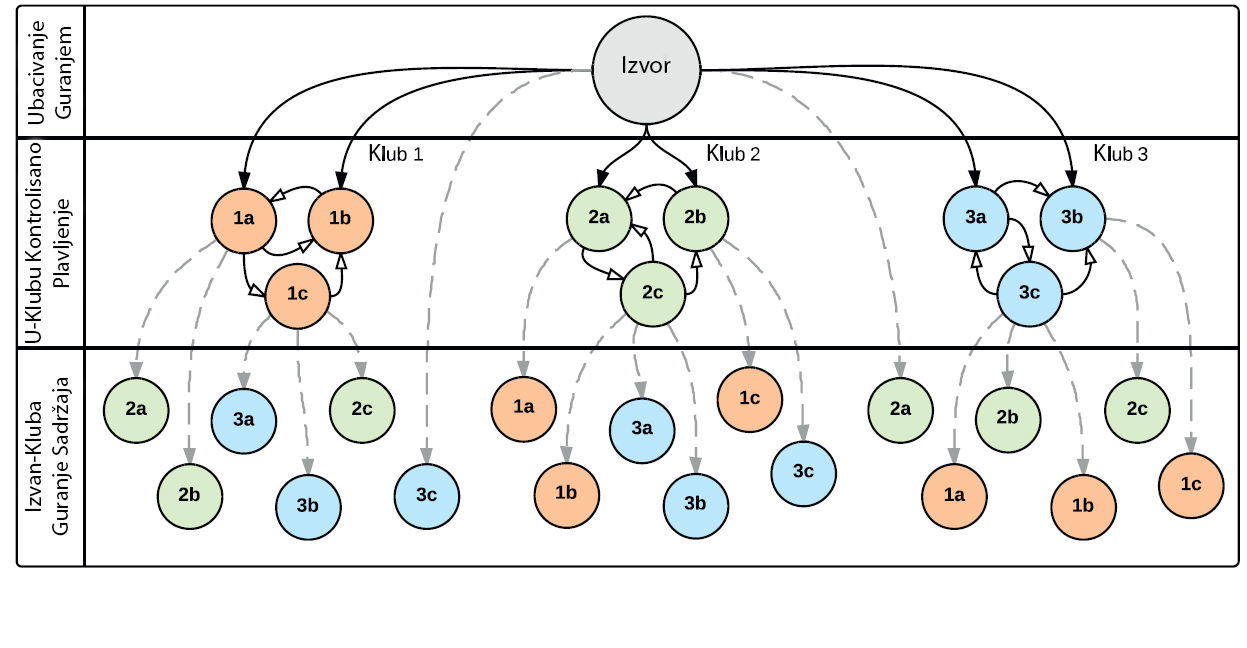
\includegraphics[width=1.05\textwidth]{slike/screamer-topology.jpg}
  \caption{Screamer topologija}
  \label{fig:screamer-topologija}
\end{figure}
\par

Protokol Kikkar je baziran na protokolu Screamer. Odavde zaključujemo da se Kikkar klasifikuje kao hibridni pokrivač koji koristi brojne mehanizme kako bi postigao što manji zastoj i dodatni saobraćaj u mreži. Na slici \ref{fig:screamer-topologija} prikazana je struktura mreže za dostavu video sadržaja u realnom vremenu za jednu konfiguraciju protokola. Uočavamo da su parnjaci podeljeni u klubove. Jedan parnjak može da pripada najviše jednom klubu. Ukupan broj klubova je 6. Proces dostave video sadržaja se može apstrahovati na tri faze: (1) ubacivanje guranjem video blokova od izvora (eng. \textit{source}) u ostale klubove, (2) kontrolisano plavljenje (eng. \textit{flooding}) u klubu, i (3) guranje sadržaja u listove mreže, tj. guranje sadržaja izvan kluba.

Kikkar protokol razlikuje tri glavne uloge u sistemu: tragač (eng. \textit{tracker}), parnjak koji proizvodi i distribuira video snimak (eng. \textit{source}) i parnjaci koji traže video snimak. Tragač služi da pomogne parnjacima u bržem i lakšem pronalaženju ostalih parnjaka. Bitno je napomenuti da se tragač koristi samo za otkrivanje novih parnjaka i sinhronizaciju časovnika u mreži. 

Kod Kikkar protokola, svi parnjaci su podeljeni u klubove, tj. svaki parnjak pripada jednom klubu. Dodeljivanje veze parnjak-klub vrši tragač prilikom pristupanja parnjaka sistemu. Parnjak doprinosi klubu kome pripada svojim resursima. Ostalim klubovima parnjak je list tj. ništa ne doprinosi već samo dobija sadržaj. Parnjak koji šalje video igra posebnu ulogu u sistemu, tj. pripada svim klubovima. Takođe, on je zadužen za podelu video snimaka na manje delove i dodelu delova određenim klubovima. Ovakav način slanja je čest kod topologije višestrukih stabala.

Parnjak komunicira sa tragačem upotrebom HTTP protokola. Parnjaci komuniciraju međusobom koristeći protokol korisničkih datagrama (eng. \textit{User Datagram Protocol, UDP}). Veze između parnjaka se formiraju tako što se povezuju parnjak koji šalje i parnjak koji prima. Važi pravilo da parnjak koji je na početku veze odabran da šalje video ne prima sadržaj od parnjaka primaoca. Drugim rečima veze su jednosmerne.  

Svaki parnjak u klubu teži da ima bar dve i ne više od tri odlazne i dolazne konekcije sa parnjacima koji pripadaju njegovom klubu. Ovim svojstvom se postiže eksponencijalna brzina slanja video snimka. Takođe, pored parnjaka iz njegovog kluba teži i da postigne po jednu dolaznu konekciju sa parnjacima koji ne pripadaju njegovom klubu. Ova konekcija je istog značaja kao i konekcija u klubu. Bez njenog postojanja, ne mogu se obezbediti svi potrebni podaci. Broj odlaznih konekcija sa parnjacima koji ne pripadaju njegovom klubu nije bitan. Konekcije će detaljnije biti opisane u pogavlju \ref{Kikkar.4}. 


\section{Pridruživanje parnjaka}
\label{Kikkar.2}

\begin{figure}[!ht]
  \centering
  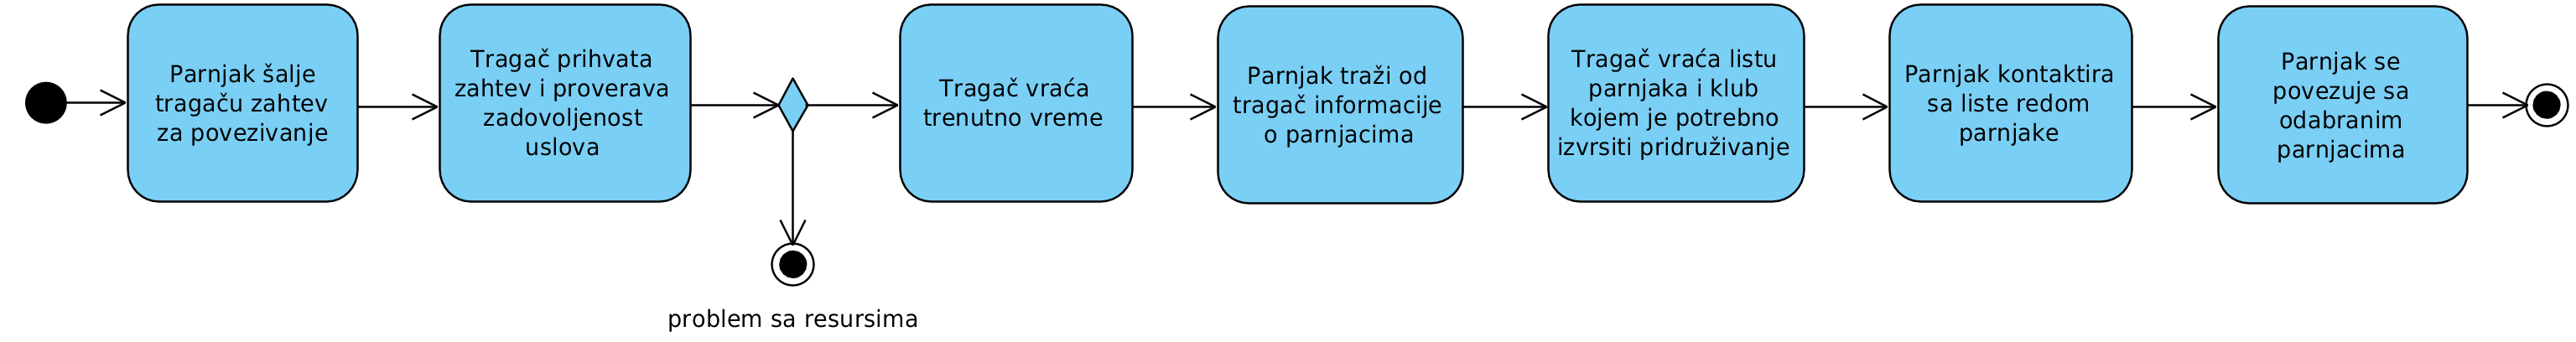
\includegraphics[width=1.05\textwidth]{slike/pridruzivanje.jpg}
  \caption{Pridruživanje novog parnjaka}
  \label{fig:pridruzivanje}
\end{figure}
\par


Prilikom pridruživanja parnjaka jatu (eng. \textit{swarm}) kako bi preuzeo sadržaj u mreži, neophodno je slanje zahteva za povezivanje tragaču. Navedeno svojstvo ilustrovano je dijagramom aktivnosti \ref{fig:pridruzivanje}. Kako bi se jato zaštitilo od pridruživanja parnjaka koji ne može obezbediti odgovarajuće resurse, tragač proverava brzinu dolaznog i odlaznog saobraćaja novog parnjaka. Ukoliko je brzina dolaznog i odlaznog saobraćaja ispod granice, tragač prekida kontakt sa parnjakom. Ukoliko je brzina dolaznog i odlaznog saobraćaja zadovoljavajuća tragač vraća trenutno vreme parnjaku korišćenjem protokola mrežnog vremena (eng. \textit{Network Time Protocol, NTP}). Nakon uspešne sinhronizacije vremena, parnjak od tragača zahteva informaciju o parnjacima koji pripadaju jatu. Tragač izdvaja iz svakog kluba određeni broj parnjaka i prosleđuje njihove informacije. Informacija sadrži IP adresu parnjaka, port na kome parnjak osluškuje i pripadnost parnjaka klubu.  Dodatno, pored informacije o parnjacima tragač prosleđuje parnjaku klub u koji je obavezan da uđe. Kako bi se obezbedio jednak broj parnjaka po klubovima, novi parnjak se uvek upućuje na prvi sledeći klub na koji je poslednji parnjak prosleđen. 


Parnjak zatim koristi dobijenu listu parnjaka kako bi odlučio sa kojima od njih će se povezati. Najpre se šalje \texttt{ping} poruka za povezivanje svim parnjacima sa liste. Ping poruka sadrži broj porta na kojem parnjak osluškuje, broj kluba u kome se parnjak nalazi i tip konekcije koju parnjak želi da ostvari tj. odlazna ili dolazna konekcija. Zatim se čekaju odgovori određeno vreme. Nakon pristizanja ping poruke, parnjak odgovara \texttt{pong} porukom koja obavezno sadrži informacije o broju veza koje ima ping-ovani parnjak i količini uskladištenih podataka. Nakon određenog vremena, parnjak pregleda primljene pong poruk i sortira parnjake prema poželjnosti. Uslov koji se koristi da bi se poredili parnjaci prema poželjnosti je količina uskladištenih podataka. U slučaju postojanja više parnjaka sa istom količinom uskladištenih podataka bira se parnjak sa što manjim brojem dolaznih ili odlaznih veza kako bi se što manje remetilo jato.
 
Zatim se odgovarajućim parnjacima šalje \texttt{request} poruka. Ova poruka sadrži informaciju o klubu u kome se parnjak trenutno nalazi kao i tip konekcije. Trenutni klub i tip konekcije su prosleđeni ranije u okviru ping poruke ali kako je moguće da parnjak u međuvremenu dobije neki drugi klub ili port ponovo se šalju. Na request poruku odgovara se \texttt{response} porukom. Response poruka predstavlja potvrdu o povezivanju. Ukoliko izostane response poruka povezivanje se i dalje smatram uspešnim pri čemu sistem za kontrolu zagušenja ima zadatak da neaktivne parnjake izbaci iz mreže. 

Svi parnjaci koji su se javili pong porukom i nisu izabrani se čuvaju u specijalnoj strukturi podataka. Glavni razlog čuvanja je brže kasnije povezivanje i manje opterećivanje servera ukoliko se kasnije ukaže potreba za povezivanjem. Parnjaci koji nisu poslali pong poruku se brišu jer se smatraju neaktivnim ili zagušenim.  


\section{Distribucija sadržaja}
\label{Kikkar.3}

\begin{figure}[!ht]
  \centering
  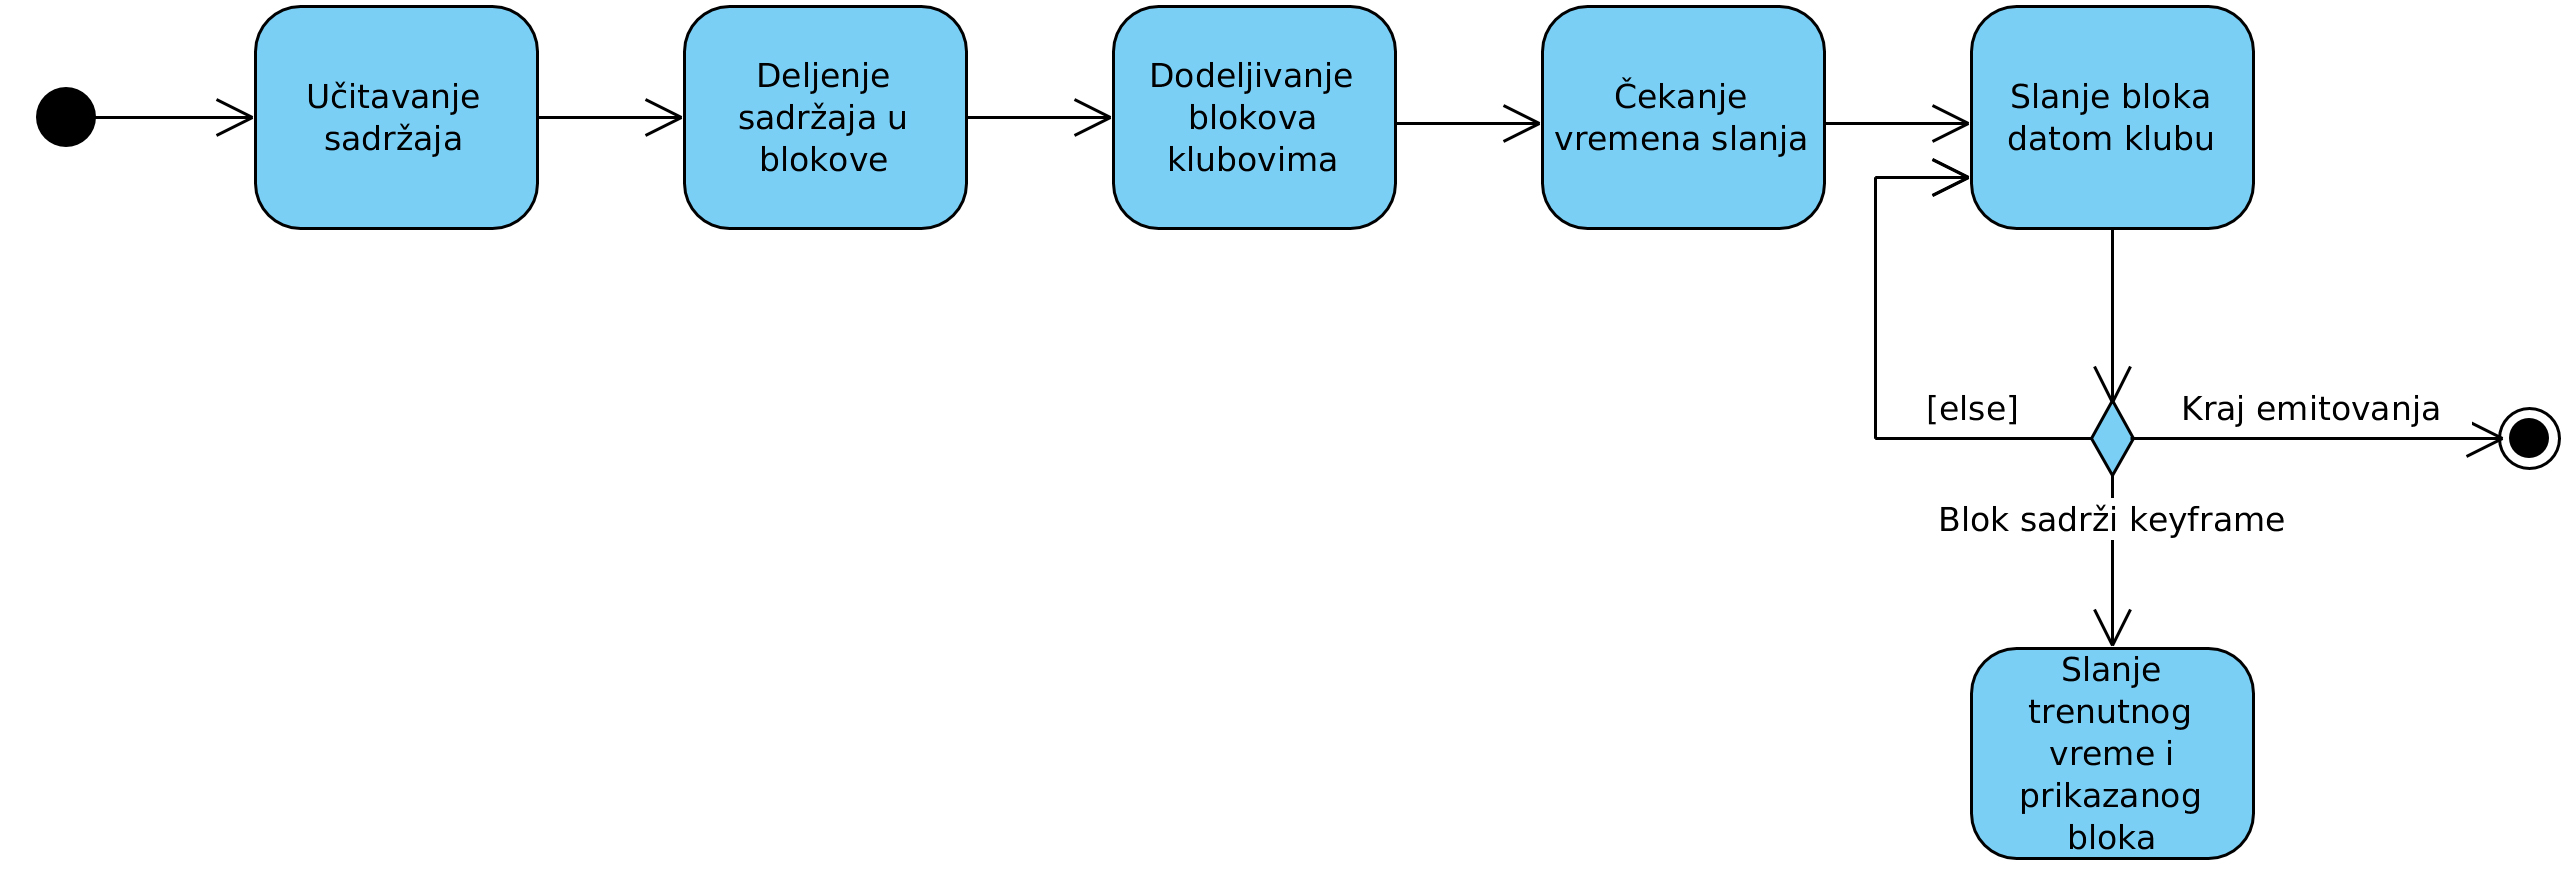
\includegraphics[width=1.05\textwidth]{slike/distribucija-izvor.jpg}
  \caption{Distribucija sadržaja od izvora ka korisnicima}
  \label{fig:distribucija-izvor}
\end{figure}
\par


U delu \ref{Kikkar.1} izvor se definiše kao parnjak koji generiše i šalje video sadržaj. Video sadržaj može biti prethodno snimljem pa samo emitovan ili uživo snimljen i emitovan. Na slici \ref{fig:distribucija-izvor} predstavljen je dijagram aktivnosti izvora. Najpre je neophodno da izvor učita sadržaj. Zatim se učitani sadržaj deli na manje blokove koji su pogodniji za prenošenje putem interneta. Svaki od blokova sadrži svoj redni broj i prema tom broju se dodeljuje jednom od klubova. Dodeljivanje se vrši tako što se redni broj podeli po modulu sa brojem klubova. Dobijeni broj odgovara broju kluba kome dati blok pripada. Dodatno, blok sadrži redni broj dela video snimka koji se šalje, informaciju da li je blok keyframe kao i sam video snimak.

Nakon dodeljivanja bloka klubu čeka se vreme slanja. Vreme čekanja odgovara ukupnom broju blokova koje je potrebno poslati podeljeno sa vremenom potrebnim za slanje blokova. Po isticanju vremena, blok se šalje u klub. Ukoliko poslati blok sadrži keyframe, pre njega se šalje \texttt{kontrolna} poruka. Kontrolna poruka sadrži broj video snimka koji je prikazan, dužinu do sada prikazanog video snimka izvora kao i vreme kada je kontrolna poruka napravljena. Osnovna svrha kontrolne poruke je da obavesti ostale parnjake u jatu o trenutno prikazanom sadržaju, tj. da omogući globalnu sinhronizaciju jata. 


\begin{figure}[!ht]
  \centering
  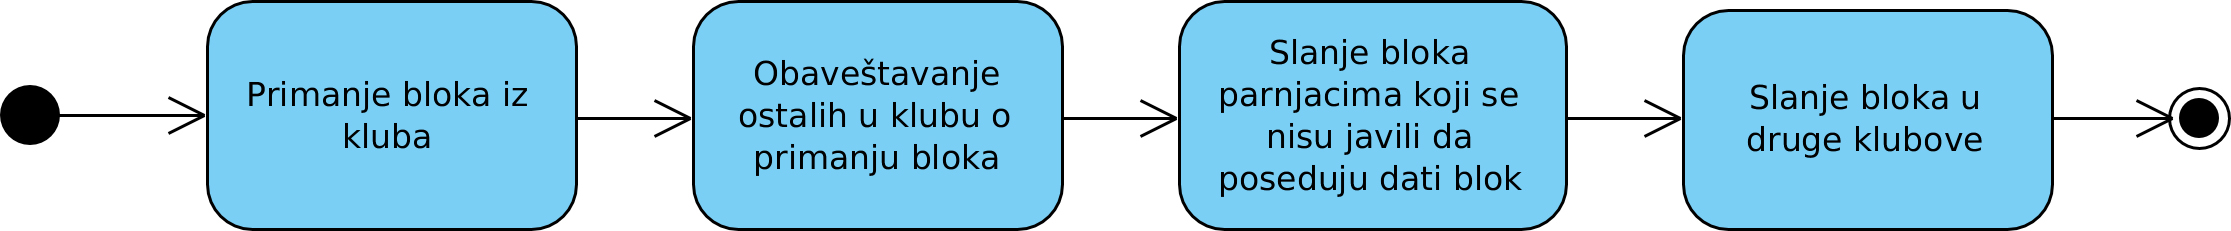
\includegraphics[width=1.05\textwidth]{slike/distribucija-jato.jpg}
  \caption{Distribucija sadržaja od izvora ka korisnicima}
  \label{fig:distribucija-izvor}
\end{figure}
\par

Kod distribucije sadržaja među korisnicima razlikujemo dva načina distribucije. Podela je izvršena u zavisnosti da li dobijeni sadržaj pripada klubu ili ne. Kada parnjak primi blok podataka koji je dodeljen njegovom klubu, on obaveštava o isporuci sve parnjake u klubu sa kojima ima odlaznu vezu a zatim snima dati blok u skladište. Obaveštenje se vrši preko \texttt{have} poruke koja sadrži broj primljenog bloka. Obaveštavanje ostalih parnjaka ima za cilj da smanji mogućnost višestruke isporuke istog sadržaja pojedinim parnjacima. Posle određenog vremena parnjak šalje sadržaj svim parnjacima od kojih nije dobio nikakvu poruku koja bi ga obavestila da već ima taj sadržaj. U poruci koja služi za obaveštenje o postojanju sadržaja nalazi se broj prisutnog bloka. Nakon što je sadržaj poslat u klub, sadržaj se šalje ostalim klubovima. Kako parnjak ima po jednu vezu sa parnjacima iz drugih klubova, nema potrebe za razmenom kontrolne poruke. Kada parnjak dobije blok koji ne pripada njegovom klubu, snima dati blok u skladište i ne distribuira blok dalje. 

Prethodno opisan metod distribucije blokova u jatu funkcioniše bez greške u idealnim uslovima.
Kako se u okviru mreže javljaju zagušenja i gube paketi, postoji mogućnost da deo snimka ne stigne do parnjaka. Da bismo obezbedili što bolji kvalitet snimka koristi se mehanizam traženja izgubljenih blokova. Pri primanju kontrolne poruke, parnjak proverava stanje prethodne grupe blokova. Za svaki nedostajući blok parnjak šalje zahtev za slanje svim komšijama u klubu. Zahtev sadrži listu brojeva nedostajućih blokova. Kako bi se izbeglo zatrpavanje komšija parnjak može tražiti najviše 20 nedostajućih blokova.
 
 
\section{Kontrola zagušenja}
\label{Kikkar.4}

U Kikkar protokolu, radi kontrolisanja zagušenja može doći do raskidanja konekcije pri određenim uslovima. Za raskidanje veze se koristi \texttt{terminirajuća} poruka. Ova poruka sadrži razlog terminacije (na primer dolazak novog parnjaka, prespora veza, izlazak iz jata). Jedna od okolnosti pri kojoj može doći do raskidanja konekcije je preveliko kašnjenje paketa. Ukoliko se preko dolazne konekcije ne dobije ni jedna poruka za unapred definisano vreme veza se smatra mrtvom i prekida se. Tačno vreme čekanja zavisi od same mreže i postavlja ga administrator mreže. Merenje vremena počinje dolaskom poslednje poruke. Pri svakoj dobijenoj poruci proveravaju se svi parnjaci. U slučaju da neki od parnjaka nije poslao poruku određeno vreme, veza se raskida. Ukoliko parnjak nema sadržaj za slanje a želi da spreči raskidanje veze, on šalje \texttt{keep-alive} poruku kojom obaveštava dobavljača sadržaja da je sa vezom sve u redu. Sa ciljem da bude što manja, keep-alive poruka sadrži samo redni broj koji je jedinstveno identifikuje. 

Druga okolnost pod kojom je dozvoljeno raskidanje veze je dolazak paketa u pogrešnom redosledu. Svaki paket ima svoj broj. Ukoliko paketi pristižu u pogrešnom redosledu to može ukazivati na postojanje zagušenja pa će paketi ići alternativnim putevima. U tom slučaju, radi rasterećenja mreže veza se raskida. Dodatno, mali broj paketa koji pristižu u pogrešnom redosledu za veći vremenski period ne mora ukazivati na kritično zagušenje. Treći način rešavanja problema sa zagušenjem je odbacivanje svih veza u kojima se blok podataka predugo čeka. Predugo čekanje obično ukazuje na usko grlo u sistemu. Radi određivanja trajanja pauze u pristizanju paketa, čuvamo vreme kada je poslednji paket primljen.

Očigledno je da odbacivanjem neke veze možemo pokvariti topologiju i da je potrebno vršiti nova povezivanja. U zavisnosti od veze koja je odbačena, zavisi da li će doći do ponovnog povezivanja. Ukoliko je parnjak izgubio dolaznu vezu van kluba, onda od tragača traži spisak parnjaka i povezuje se sa parnjakom iz istog kluba kome je pripadao parnjak čija je veza izgubljena. Povezivanje se vrši postupkom koji je opisan u delu \ref{Kikkar.2}. Ukoliko je parnjak izgubio odlaznu vezu van kluba, ne vrši se nikakvo povezivanja. U slučaju da su parnjaci u istom klub, stvari su komplikovanije. U slučaju da parnjak izgubi dolaznu vezu u klubu, proverava da li su mu ostale najmanje još dve dolazne veze. Ukoliko nisu pronalazi se novi parnjak i vrši se povezivanje koje je opisano u delu \ref{Kikkar.2}. Isti princip važi i u slučaju gubljenja dolazne veze.

Pored problema sa manjkom veza, može se javiti i višak veza parnjaka. Kada parnjak dobije zahtev za povezivanje, povezivanje se ostvaruje ne uzimajući u obzir prethodne veze. Ukoliko parnjak ima više od tri dolazne ili tri odlazne veze u klubu potrebno je neke veze odbaciti. Odbacuju se one veze koje najduže nisu prenele paket. 
  

\section{Sinhronizacija parnjaka}
\label{Kikkar.5}

\begin{figure}[!ht]
  \centering
  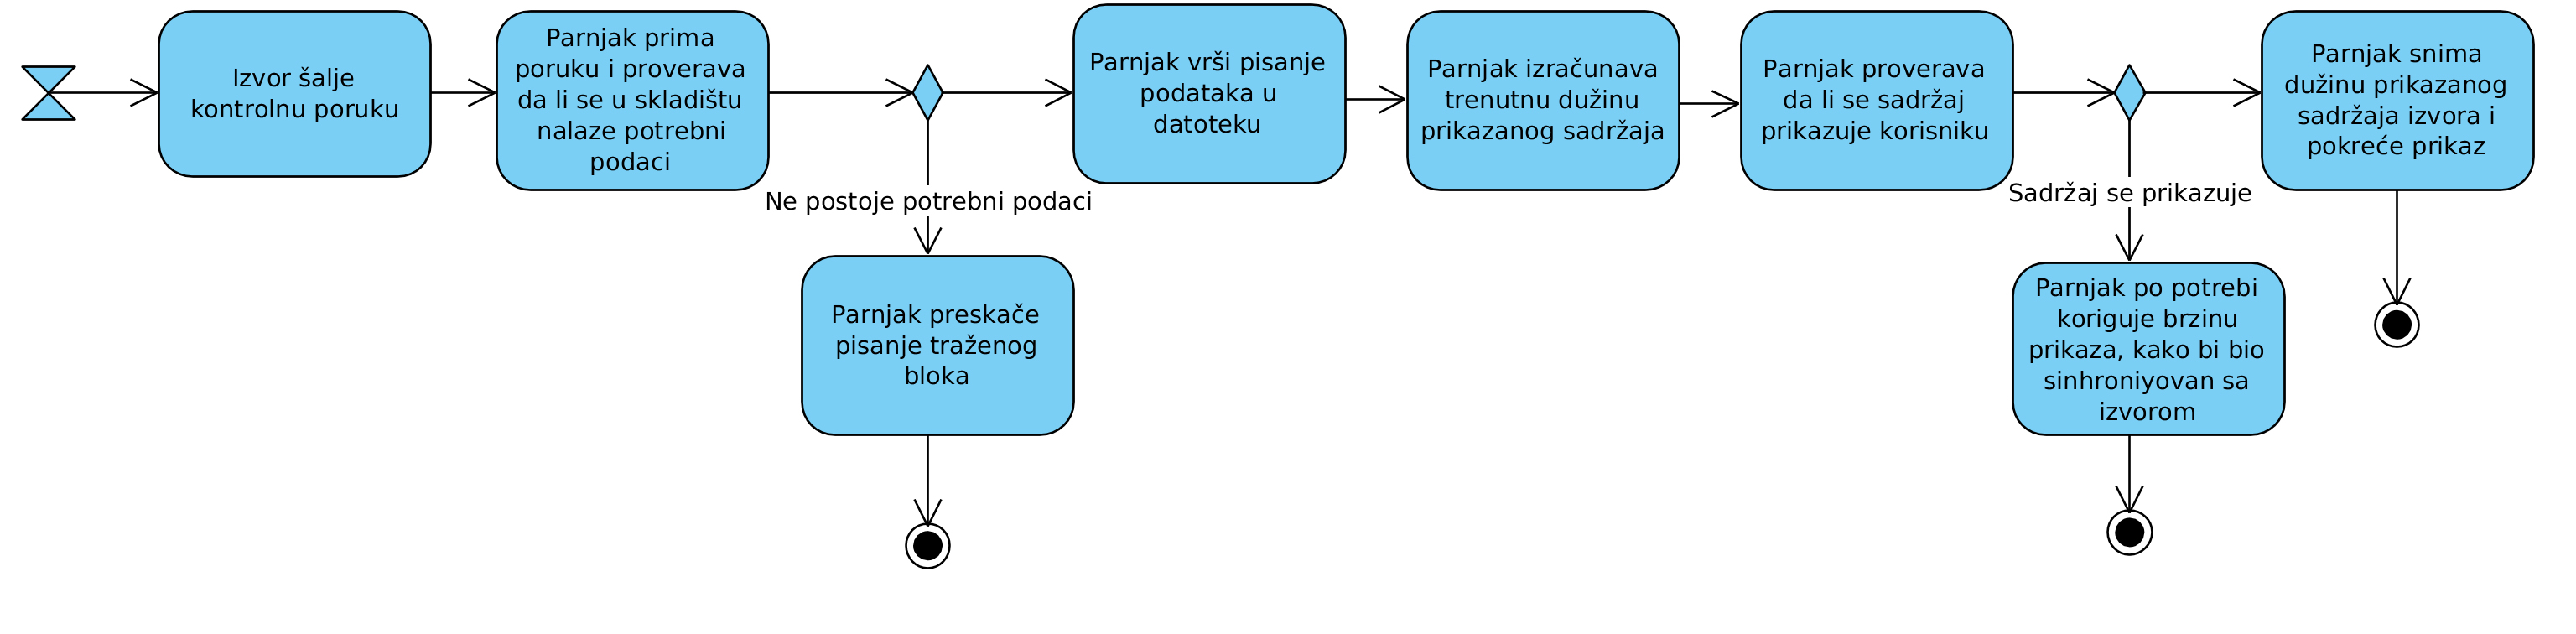
\includegraphics[width=1.05\textwidth]{slike/sinhronizacija.jpg}
  \caption{Sinhronizacija sadržaja}
  \label{fig:sinhronizacija}
\end{figure}
\par

U Kikkar protokolu izvor je pored slanja video sadržaja zadužen i za slanje kontrolnih poruka. Na slici \ref{Kikkar.5} ilustrovan je način obrade kontrolne poruke. Kontrolna poruka se šalje u pravilnim razmacima pre svakog keyframe-a. Za razliku od ostalih poruka, kontrolna poruka se zbog svoje važnosti šalje u sve klubove. Nakon primanja kontrolne poruke, parnjak je prosleđuje svim komšijama sa kojima ima odlaznu vezu, bez obzira da li su je oni već primili i da li su u njegovom klubu. Na ovaj način se osigurava da poruka stigne do svakog parnjaka. Nakon primanja kontrolne poruke koja ima isti sadržaj kao i neka od prethodnih poruka parnjak prekida njeno dalje prosleđivanje. Na ovaj način se sprečava beskonačno slanje poruke kroz jato. Nakon primanja kontrolne poruke, parnjak proverava da li skladište sadrži odgovarajuće video blokove koji su porukom obuhvaćeni. Ukoliko skladištu nedostaje prvi obuhvaćeni blok, preskače se ceo opseg. Kako se sve značajne informacije za prikazivanje video snimka nalaze u prvom bloku, prethodna činjenica je potpuno opravdana. U slučaju postojanja prvog bloka, obuhvaćeni blokovi se šalju video plejeru. Kako bi se sprečilo prekidanje video snimka, u slučaju preskakanja nekog video bloka prikazuje se prethodni video blok.

Ukoliko je uspešno izvršeno slanje sadržaja video plejeru, prelazi se na korak sinhronizacije. U koraku sinhronizacije se proverava da li video plejer prikazuje sadržaj. U slučaju neaktivnosti multimedijalnog plejera, snima se vrednost prikazanog sadržaja izvora sabrana sa kašnjenjem paketa. Ova vrednost će se koristiti kasnije kao reper za eventualne korekcije. Nakon što je vrednost snimljena pokreće se multimedijalni plejer. Ukoliko je plejer već aktivan, izračunava se dužina do sada prikazanog sadržaja. Ukoliko je ta dužina manja od zbira dužine emitovanja sadržaja izvora i kašnjenja paketa, potrebno je povećati brzinu snimka određeni vremenski interval dok se ne sinhronizuje sa izvorom. Slično, u slučaju da je pomenuta dužina veća od zbira dužine emitovanja sadržaja izvora i kašnjenja paketa, brzina se smanjuje određeni vremenski interval dok se ne postigne sinhronizacija sa izvorom. 


\chapter{Implementacija Kikkar protokola}
\label{chp:p2p-implementacija}

Za demonstraciju Kikkar protokola opisanog u poglavlju \ref{chp:p2p-protokol} razvijene su veb i desktop aplikacija. Za razvoj je korišćen programski jezik Java 8 \cite{Java} i razvojno okruženje Eclipse \cite{Eclipse}. Veb aplikacija implementira funkcionalnosti tragača Kikkar protokola, a desktop aplikacija u zavisnosti od podešenih parametara predstavlja parnjaka ili izvor. 

Za uspešno pokretanje veb aplikacije neophodan je Java servlet kontejnera (eng. \textit{Java Servlet Container}), dok je za desktop aplikaciju potrebna samo Java virtuelna mašina (eng. \textit{Java virtual machine, JVM}). Prilikom inicijalizacije desktop aplikacije bira se mod pokretanja aplikacije. Dostupni su mod izvora ili mod parnjaka. Kada je mod izabran, aplikacija do kraja rada ostaje u odabranom modu. I veb i desktop aplikacija su otvorenog koda i mogu se pronaći na github repozitorijumu \footnote{Repozitorijum se može naći na adresi \url{https://github.com/ozzy80/master-rad/tree/master/kod}}. Detaljnije o veb aplikaciji može se pronaći u poglavlju \ref{implementacija.1}. Više detalja o desktop aplikaciji nalazi se u poglavlju \ref{implementacija.2}.

\section{Implementacija tragača}
\label{implementacija.1}

Implementacija Kikkar protokola obuhvata aplikacije za veb i desktop. Veb aplikacija predstavlja tragača Kikkar protokola. 


Pre implementacije samog tragača, neophodno je obavljanje nekoliko zadataka.
Prvi zadatak je odabir odgovarajućeg Java servlet kontejnera za izvršavanje veb aplikacije. Za Java servlet kontejner odabran je Tomcat \cite{Tomcat} verzije 9. Razlozi za odabir Tomcat kontejnera su široka primena u industriji, jednostavnost, odlična zajednica i dokumentacija. Drugi zadatak je odabir odgovarajuće baze podataka. Za bazu podataka izabrana je MySQL \cite{Mysql} baza. Detaljnije o samoj bazi i formiranim tabelama nalazi se u poglavlju \ref{implementacija.1.1}. Konačno, potrebno je naći odgovarajće radne okvire (eng. \textit{framework}). Detaljnije o korišćenim bibliotekama i radnim okvirima može se pronaći u poglavlju \ref{implementacija.1.2}. U poglavlju \ref{implementacija.1.3} dat je opis funkcionalnosti aplikacije.

\subsection{Baza podataka}
\label{implementacija.1.1}

Za potrebe aplikacije izabrana je MySQL \cite{Mysql} baza podataka. Razlog za odabir MySQL baze podataka je široka primena u industriji i nauci, dobra dokumentacija i jednostavna integracija. Na slici \ref{fig:eer} predstavljen je EER dijagram baze podataka (eng. \textit{EER database diagram}). 

\begin{figure}[!ht]
  \centering
  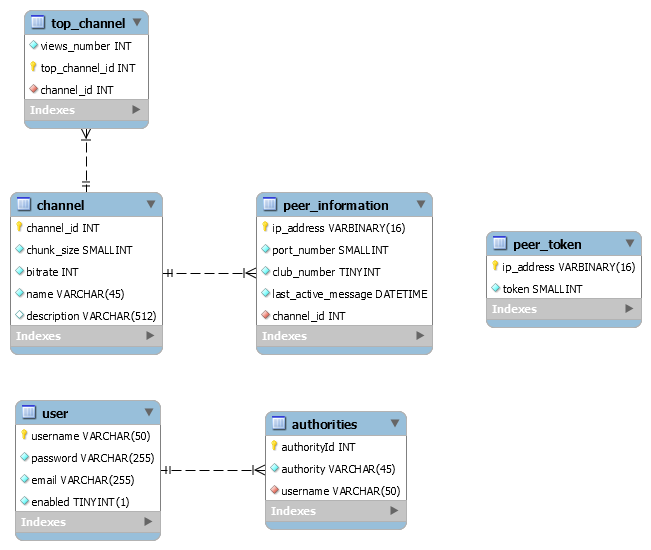
\includegraphics[width=1.05\textwidth]{slike/eer-dijagram.png}
  \caption{EER dijagram baze podataka}
  \label{fig:eer}
\end{figure}
\par


Tabela \texttt{channel} sadrži informacije o kanalima. Ove informacije pruža emiter signala pri registraciji kanala. Informacije koje se čuvaju u tabeli obuhvataju:

\begin{center}
\begin{tabular}{ p{3.8cm} p{10.2cm} }
 \textit{channel\_id} & - jedinstveni identifikacioni broj kanala, primarni ključ \\ 
 \textit{chunk\_size} & - maksimalnu veličinu bloka podatka poslatog kroz mrežu \\  
 \textit{bitrate} & - maksimalnu brzinu protoka video snimka \\
 \textit{name} & - ime kanala \\
 \textit{description} & - opis kanala \\
\end{tabular}
\end{center}


Tabela \texttt{peer\_information} čuva informacije o aktivnim parnjacima za svaki kanal posebno. Za svakog parnjaka čuva se:

\begin{center}
\begin{tabular}{ p{3.8cm} p{10.2cm} }
 \textit{ip\_address} & - IP adresa, primarni ključ \\ 
 \textit{port\_number} & - broj porta na kojem se osluškuje saobraćaj \\  
 \textit{club\_number} & - broj kluba kojem pripada \\
 \textit{last\_active\_message} & - vreme poslednje primljene aktivne poruke \\
 \textit{channel\_id} & - jedinstven identifikacioni broj gledanog kanala, strani ključ ka tabeli \texttt{channel} \\
\end{tabular}
\end{center}


Tabela \texttt{user} čuva informacije o vlasnicima kanala, izvornim parnjacima. Tabela sadrži navedena polja:

\begin{center}
\begin{tabular}{ p{3.8cm} p{10.2cm} }
 \textit{username} & - jedinstveno korisničko ime, primarni ključ \\ 
 \textit{password} & - šifru korisnika \\  
 \textit{email} & - email adresa korisnika \\
 \textit{enabled} & - podatak o odobrenosti naloga \\
\end{tabular}
\end{center}

Tabela \texttt{authorities} služi za autorizaciju korisnika. Sastoji se od polja:

\begin{center}
\begin{tabular}{ p{3.8cm} p{10.2cm} }
 \textit{authority\_id} & - jedinstveni broj autorizacije, primarni ključ \\ 
 \textit{authority} & - ime autorizacije \\  
 \textit{username} & - jedinstveno korisničko ime, strani ključ ka tabeli \texttt{user} \\
\end{tabular}
\end{center}

Tabela \texttt{top\_channel} čuva listu najposećenijih kanala. Tabela se sastoji od polja:
 
\begin{center}
\begin{tabular}{ p{3.8cm} p{10.2cm} }
 \textit{views\_number} & - broj aktivnih parnjaka \\ 
 \textit{top\_channel\_id} & - jedinstveni identifikacioni broj, primarni ključ \\  
 \textit{channel\_id} & - jedinstven identifikacioni broj kanala, strani ključ ka tabeli \texttt{channel}  \\
\end{tabular}
\end{center}


Tabela \texttt{peer\_token} služi za čuvanje dodeljenog pristupnog tokena korisnicima. Tabela se sastoji od polja: 

\begin{center}
\begin{tabular}{ p{3.7cm} p{10.3cm} }
 \textit{ip\_address} & - IP adresa parnjaka, primarni i strani ključ ka tabeli \texttt{user}\\ 
 \textit{tokena} & - pristupni token \\
\end{tabular}
\end{center}


\subsection{Korišćene biblioteke i radni okviri}
\label{implementacija.1.2}

Pre opisa korišćenih biblioteka i radnih okvira, ukratko će biti predstavljen softverski alat \textit{Apache Maven} \cite{Maven}. Glavna namena alata je upravljanje i izgradnja projekta. Dva osnovna pravca upotrebe su priprema izvornog koda za distribuciju i jednostavno dodavanje Java biblioteka (eng. \textit{jars}) u projekat. Kako su Java biblioteke obimne, većinom se nove biblioteke grade korišćenjem već postojećih. Postojeće biblioteke često koriste druge biblioteke pri čemu pomenuta zavisnost može biti proizvoljne dubine. U slučaju nekompatibilnosti različitih verzija biblioteka zadatak se dodatno komplikuje.
Pri upotrebi Apache Maven alata pravila o zavisnostima navodimo u datoteci \textit{pom.xml}. Ova datoteka mora da sadrži grupu, predmet za upotrebu, verziju i naziv projekta. U okviru pom.xml datoteke definiše se i način pakovanja, koji može biti jar (eng. \textit{Java Application Archive}) ili war (eng. \textit{Web Application Archive}). Kako je tragač veb aplikacija koristi se war. U okviru pom.xml nalazi se i deo sa zavisnostima (eng. \textit{dependencies}). U okviru ovog dela se definišu biblioteke ili radni okviri koji su neophodni projektu. Bez upotrebe Maven-a navedena pravila morala bi se ručno postavljati. 

U nastavku će biti opisane korišćene biblioteke i radni okviri. Prvi korišćeni je \textit{Spring} radni okvir \cite{Spring}.
Spring je nastao 2002. godine sa idejom omogućavanja lake manipulacije velikih projekata na Java platformi (eng. \textit{Java SE}). Pre Spring-a koristila se najčešće čista Java (eng. \textit{pure Java}). Glavna mana ovakvog pristupa je težina učenja i održavanja koda. U početku Spring je predstavljao dopunu Java standarda za poslovne aplikacije (eng. \textit{Java 2 Platform Enterprise Edition, J2EE}), ali danas se sve više koristi kao alternativa preobimnom i kompleksnom J2EE standardu, naročito u delu koji se tiče rada sa Java zrnima (eng. \textit{Enterprise Java Beans}). Spring se može koristiti u bilo kojoj Java aplikaciji. Kao projekat, Spring okvir sastoji se od više modula koji su u velikoj meri nezavisni, tako da svaka aplikacija može da koristi samo deo Spring okvira koji joj je potreban. U projektu je korišćeno jezgro Springa, koje je obavezno za sve Spring okvire, modul podrške za veb MVC (eng. \textit{Model–view–controller, MVC}) radni okvir, objektno relaciono mapiranje (eng. \textit{object relational mapping}) i sigurnost same veb aplikacije.

Prilikom razvoja korisničke aplikacije jedna od ključnih stvari je razdvajanje sadržaja od prezentacije. Kako bismo ovo postigli na veb-u koristimo MVC arhitekturu. Glavni akcenat ovakve arhitekture je podela odgovornosti između različitih slojeva. Aplikacija je podeljena na tri glavne komponente i svaka od njih obavlja različite zadatke. Model je prva komponenta. On predstavlja internu reprezentaciju podataka. Sadrži glavne programske podatke kao što su informacije o objektima iz baze. Druga komponenta je pogled. Ova komponenta omogućava korisniku interfejs preko kog može da komunicira sa aplikacijom i prikazuje korisniku stanje modela. Treća komponenta je kontrolor. Glavna odgovornost kontrolora je upravljanje korisničkim zahtevima i iniciranje aktivnosti na nivou modela i promene na pogledu. 

Komunikacija sa bazom podataka urađena je uz pomoć Hibernate \cite{Hibernate}. Hibernate je programski okvir za objektno-relaciono mapiranje u Java programskom jeziku. Njegova glavna svrha je mapiranje objektno-orijentisanog modela u model relacione baze podataka radi lakše manipulacije podacima i održavanja koda. Mapiranje se postiže povezivanjem Java klasa i tabela baze podataka i mapiranjem Java tipova podataka u SQL tipove podataka. Povezivanje Java klasa i tabela baze podataka vrši se korišćenjem Java anotacija. Pretraga upita vrši se uz pomoć objektno orijentisane verzije SQL-a koja se zove HQL (eng. \textit{Hibernate Query Language, HQL}). HQL nam omogućava pisanje upita nad Java objektima, a to znači da su upiti nezavisni od tipa baze podataka. Ukoliko projekat zahteva promenu tipa baze podataka, neće biti potrebe za menjanjem upita unutar projekta. Za sam pristup MySQL bazi koristi se MySQL konektor. 

Za kreiranje i čitanje iz JSON formata koristi se \textit{jackson} \cite{Jackson}. Jackson je veoma popularna i izuzetno efikasna Java biblioteka za serijalizaciju i mapiranje Java objekata u JSON i obrnuto. Ostale biblioteke koje se koriste su \textit{jstl} \cite{JSTL} kao tehnologija za kreiranje veb stranica sa dinamičkim sadržajem, biblioteka \textit{bootstrap} \cite{Bootstrap} za kreiranje responzivnih veb sadržaja i \textit{JQuery} \cite{JQuery} kao biblioteka za brži i lakši razvoj interaktivne veb stranice. 


\subsection{Neki detalji implementacije}
\label{implementacija.1.3}

Pri implementaciji tragača koristi se MVC arhitektura. Model čine klase \texttt{Channel}, \texttt{Authorities}, \texttt{PeerInformation}, \texttt{Token}, \texttt{TopChannel} i \texttt{User} koje redom odgovaraju istoimenim tabelama iz poglavlja \ref{implementacija.1.2}. Sloj za pristup objektima (eng. \textit{data access object, DAO}) služi za pisanje jednostavnih HQL naredbi za pristup mapiranim objektima. Klase koje se nalaze u ovom sloju imaju identična imena kao modeli kojim pristupaju sa nastavkom DAO. Sloj servisa služi za biznis logiku. Sastoji se od klasa \texttt{ChannelManager}, \texttt{PeerConnectionManager}, \texttt{PeerInformationManager}, \texttt{TokenManager} i \texttt{UserManager}. Većina metoda ovih klasa vrši prosleđivanje upita nižim slojevima, jer ne postoji nikakva logika koju bi bilo neophodno implementirati. Jedini izuzetak je metod \textit{void deleteDeadPeers()} koji je privatan u klasi \texttt{PeerInformationManager} i koristi se za periodično brisanje parnjaka koji se nisu javili u poslednjih 1000 sekundi. Kontroler se sastoji od klasa \texttt{FileUploadController}, \texttt{HomeController}, \texttt{LoginController} i \texttt{PeerConnectionController}. Za preuzimanje fajlova od korisnika koristi se klasa \texttt{FileUploadController}. \texttt{LoginController} se koristi za prijavljivanje i kreiranje novih naloga emiterima video sadržaja.
Za opsluživanje veb stranica koristi se \texttt{HomeController}. Za pristupanje parnjacima koristi se \texttt{PeerConnectionController}.

Serverska aplikacija je napravljena po REST principima i prihvata zahteve ka
sledećim adresama:


\begin{center}
\begin{tabular}{ |p{1.5cm}|p{4cm}|p{8cm}| } 
\hline
Metoda & Putanja & Opis \\
\hline
\texttt{POST} & \texttt{/channel/fileUpload} & Prihvata sliku od klijenta i čuva je u bazi podataka \\
\texttt{GET} & \texttt{/} & Preusmerava korisnika na stranicu za prijavljivanje \\ 
\texttt{GET} & \texttt{/channel} & Provera da li je korisnik prijavljen. Ukoliko jeste šalje ga na stranicu sa kanalima, ukoliko nije vraća ga na formu za prijavljivanje \\ 
\texttt{GET} & \texttt{/channel/{channelId}} & Vraća podatke o kanalu čiji je jedinstveni identifikacioni broj \texttt{{channelId}}\\
\texttt{GET} & \texttt{/login} & Preusmerava korisnika na stranu za prijavljivanje \\ 
\texttt{POST} & \texttt{/register} & Prihvata podatke od korisnika i čuva ih u bazi podataka, preusmerva korisnika na stranicu sa spiskom kanala \\ 
\texttt{GET} & \texttt{/initial/{channelId}} & Proverava se korisnikova verzija protokola. Ukoliko nije podržana vraća se statusni kod 505, ukoliko jeste proverava se brzina odlaznog i dolaznog saobraćaja. Ukoliko je brzina zadovoljavajuća prosleđuje se pristupni token, ukoliko nije vraća se statusni kod 509 \\ 
\texttt{GET} & \texttt{/list/{channelId}} & Proverava se dobijeni token. Ukoliko token nije validan vraća se statusni kod 412, u suprotnom vraća se lista parnjaka \\ 
\texttt{GET} & \texttt{/leave} & Parnjak se briše iz liste parnjaka \\ 
\texttt{GET} & \texttt{/stayAlive} & Postavlja se vreme poslednjeg javljanja parnjaka \\ 
\hline
\end{tabular}
\end{center}


\section{Implementacija parnjaka}
\label{implementacija.2}

U poglavlju \ref{implementacija.1} opisan je tragač kao jedan deo Kikkar protokola. U ovom poglavlju opisuje se desktop aplikacija. Desktop aplikacija odgovara parnjaku Kikkar protokola. U zavisnosti od podešenog moda parnjak može biti izvor ili obični parnjak. Za implementaciju parnjaka korišćeni su razni radni okviri i biblioteke. Detaljniji opisi radnih okvira i biblioteka nalaze se u poglavlju \ref{implementacija.2.1}. Kako bi jato moglo da funkcioniše razmenjuju se poruke između parnjaka. Detaljnije o tipu i nameni svake poruke može se naći u poglavlju \ref{implementacija.2.2}. U poglavlju \ref{implementacija.2.3} dat je opis funkcionalnosti koje aplikacija pruža.

\subsection{Korišćene biblioteke i radni okviri}
\label{implementacija.2.1}

Za upravljanje i izgradnju projekta koristi se \textit{Apache Maven} \cite{Maven} koji je opisan u poglavlju \ref{implementacija.1.2}. 

Biblioteka \textit{Apache Commons Net} \cite{CommonsNet} se koristi za NTP protokol. Ona je skup različitih implementiranih internet protokola na klijentskoj strani. Glavna svrha biblioteke je da omogući korišćenje različitih protokola. Bitno je napomenuti da ona ne obezbeđuje viši nivo apstrakcije protokola već samo implementaciju.  

Za pisanje jediničnih testova u projektu koriste se radni okviri \textit{JUnit} \cite{Junit} i \textit{Mockito} \cite{Mockito}. JUnit dinamički proverava ispravnost softvera izvođenjem konačnog broja testova i upoređivanjem dobijenih rezultata sa očekivanim ponašanjem softvera. Koristi se za testiranje jedinica koda i integraciono testiranje. Testiranje jedinica koda je testiranje gde se svaka jedinica koda zasebno testira, pri čemu jedinica koda može biti funkcija, metod, klasa, operacija, struktura podataka u zavisnosti od konteksta i programske paradigme. Integraciono testiranje je testiranje tokom kojeg se proverava saradnja između modula koji predstavljaju jednu celinu sistema. U okviru projekta je korišćeno samo testiranje jedinica koda. Mockito je radni okvir koji omogućava kreiranje duplih test objekata (eng. \textit{test double objects (mock objects)}) u automatskom jediničnom testiranju. Glavna korist od duplih test objekata je obmotavanje objekta tako da pri svakom pozivu vrši unapred definisanu akciju.

\textit{Gson} \cite{Gson} je Google-ova biblioteka koja se koristi za konverziju Java objekata u njihovu JSON reprezentaciju i obrnuto. Glavna prednost Gson-a nad sličnim bibliotekama je ta što radi sa proizvoljnim objektima. Navedena činjenica omogućava konvertovanje objekata u JSON reprezentaciju čak i ako nemamo njihov izvorni kod (eng. \textit{source code}). Takođe, Gson potpuno podržava Java dženerike (eng. \textit{Java Generics}), što često nije slučaj sa sličnim bibliotekama.

Za potrebe pozivanja metoda prema unapred određenom rasporedu koristi se biblioteka otvorenog koda \textit{Quartz} \cite{Quartz}. Quartz je veoma moćna biblioteka koja se može koristiti kako za jednostavne tako i za komplikovane zadatke. Glavna prednost biblioteke Quartz nad drugim bibliotekama iste namene je što sa lakoćom može obraditi i održavati i desetine hiljada poslova. 

Za formatiranje poruka koje se razmenjuju među parnjacima koristi se Google-ova biblioteka \textit{Protocol buffers} \cite{ProtocolBuffers}. Protocol buffers je biblioteka koja se koristi za binarnu serijalizaciju podataka. Biblioteka radi tako što se definiše struktura podataka koje želimo da serijalizujemo. Kada je struktura definisana vrši se prevođenje definisane strukture u odgovarajući programski jezik. Definisana struktura podataka omogućava da se razmenjuju podaci između različitih programskih jezika. Pošto se prenose binarni podaci dobijeni izlaz je značajno brži i manji od izlaza dobijenog primenom tekstualnih formata kao što su XML ili JSON format. Detaljnije o porukama koje se koriste u protokolu može se pronaći u poglavlju \ref{implementacija.2.2} 

Za video plejer izabran je \textit{VLC} plejer \cite{VLC} zbog dobre podrške, dokumentacije i velikog izbora kodeka. Da bi VLC plejer mogao koristiti iz Java aplikacije upotrebljava se programski okvir VLCj \cite{VLCJ}. VLCj omogućava Java aplikaciji da pokrene instancu nativnog VLC medijskog plejera u okviru Java AWT prozora ili Swing JFrame-a.


\subsection{Protocol buffers poruke}
\label{implementacija.2.2}

Kao što je navedeno u poglavlju \ref{implementacija.2.1} za razmenu poruka se koristi biblioteka Protocol buffers. Protocol buffers je izabran u mnoštvu sličnih biblioteka jer je izlaz dobijen primenom ove biblioteke mali, sama biblioteka je dobro dokumentovana i jednostavna za korišćenje i ima odličnu zajednicu. U nastavku sledi opis svake poruke koja se razmenjuje u okviru Kikkar protokola.


\lstinputlisting[language=protobuf2,style=protobuf,caption={Enumeracija tipova konekcije},label=ConnectionType]{messages/ConnectionType.proto}

Enumeracija tipova konekcije predstavljena kodom \ref{ConnectionType} sadrži informaciju o tipu konekcije koju parnjak želi da ostvari. Postoje tri tipa konekcije: dolazna (\textit{DOWNLOAD}), odlazna (\textit{UPLOAD}) i oba (\textit{BOTH}). Ukoliko parnjak želi odlaznu konekciju znači da traži parnjaka kome će prosleđivati sadržaj. Ukoliko parnjak traži dolaznu konekciju znači da traži parnjaka od koga će dobijati sadržaj. U slučaju da parnjak zahteva oba tipa konekcije znači da će kasnije odlučiti koji će tip konekcije koristiti.


\lstinputlisting[language=protobuf2,style=protobuf,caption={Ping poruka},label=PingMessage]{messages/PingMessage.proto}

\textit{Ping poruka} predstavljena kodom \ref{PingMessage} definiše ping poruku opisanu u poglavlju \ref{Kikkar.2}. Poruka se sastoji od:
 
\begin{center}
\begin{tabular}{ p{4cm} p{10cm} }
 \textit{pingId} & - jedinstveni identifikacioni broj poruke \\ 
 \textit{portNumber} & - broj porta na kome se osluškuje saobraćaj \\  
 \textit{clubNumber} & - broj pripadajućeg kluba \\
 \textit{connectionType} & - tip  tražene konekcije \\
\end{tabular}
\end{center}


\lstinputlisting[language=protobuf2,style=protobuf,caption={Pong poruka},label=PongMessage]{messages/PongMessage.proto}

\textit{Pong poruka} predstavljena kodom \ref{PongMessage} definiše pong poruku opisanu u poglavlju \ref{Kikkar.2}. Poruka se sastoji od:
 
\begin{center}
\begin{tabular}{ p{4cm} p{10cm} }
 \textit{responsePingId} & - jedinstveni identifikacioni broj ping poruke na koju se odgovara \\ 
 \textit{uploadLinkNum} & - broj odlaznih veza \\  
 \textit{downloadLinkNum} & - broj dolaznih veza \\
 \textit{bufferVideoNum} & - broj uskladištenog video sadržaja \\
\end{tabular}
\end{center}


\lstinputlisting[language=protobuf2,style=protobuf,caption={Request poruka},label=RequestMessage]{messages/RequestMessage.proto}

\textit{Request poruka} predstavljena kodom \ref{RequestMessage} definiše request poruku opisanu u poglavlju \ref{Kikkar.2}. Poruka se sastoji od:
 
\begin{center}
\begin{tabular}{ p{4cm} p{10cm} }
 \textit{requestId} & - jedinstveni identifikacioni broj poruke \\ 
 \textit{clubNumber} & - broj pripadajućeg kluba \\  
 \textit{connectionType} & - tip  tražene konekcije \\
\end{tabular}
\end{center}


\lstinputlisting[language=protobuf2,style=protobuf,caption={Response poruka},label=ResponseMessage]{messages/ResponseMessage.proto}

\textit{Response poruka} \ref{ResponseMessage} predstavlja response poruku opisanu u poglavlju \ref{Kikkar.2}. Poruka se sastoji od:
 
\begin{center}
\begin{tabular}{ p{4cm} p{10cm} }
 \textit{responseRequestId} & - jedinstveni identifikacioni broj request poruke na koju se odgovara \\ 
\end{tabular}
\end{center}


\lstinputlisting[language=protobuf2,style=protobuf,caption={Response poruka},label=VideoPacket]{messages/VideoPacket.proto}

\textit{Video paket} poruka predstavljena kodom \ref{VideoPacket} definiše video snimak koji se šalje kroz jato. Poruka se sastoji od:
 
\begin{center}
\begin{tabular}{ p{4cm} p{10cm} }
 \textit{videoNum} & - jedinstveni identifikacioni broj video snimka \\ 
 \textit{chunkNum} & - broj dela snimka \\ 
 \textit{firstFrame} & - identifikator prvog frejma snimka \\ 
 \textit{video} & - video sadržaj \\ 
\end{tabular}
\end{center}


\lstinputlisting[language=protobuf2,style=protobuf,caption={Kontrolna poruka},label=ControlMessage]{messages/ControlMessage.proto}

\textit{Kontrolna poruka} predstavljena kodom \ref{ControlMessage} je kontrolna poruka opisana u poglavlju \ref{Kikkar.5}. Poruka se sastoji od:
 
\begin{center}
\begin{tabular}{ p{4.5cm} p{9.5cm} }
 \textit{messageId} & - jedinstveni identifikacioni broj poruke \\ 
 \textit{currentChunkVideoNum} & - trenutno prikazani video blok \\ 
 \textit{playerElapsedTime} & - prošlo vreme od početka emitovanja snimka \\ 
 \textit{timeInMilliseconds} & - vreme pravljenja poruke \\ 
\end{tabular}
\end{center}


\lstinputlisting[language=protobuf2,style=protobuf,caption={Have poruka},label=HaveMessage]{messages/HaveMessage.proto}

Poruka \textit{HaveMessage} predstavljena kodom \ref{HaveMessage} je have poruka opisana u poglavlju \ref{Kikkar.3}. Poruka se sastoji od:
 
\begin{center}
\begin{tabular}{ p{4.5cm} p{9.5cm} }
 \textit{videoNum} & - broj primljenog video bloka \\ 
\end{tabular}
\end{center}


\lstinputlisting[language=protobuf2,style=protobuf,caption={NotInterested poruka},label=NotInterestedMessage]{messages/NotInterestedMessage.proto}

Poruka \textit{NotInterestedMessage} predstavljena kodom \ref{NotInterestedMessage} je notInterested poruka opisana u poglavlju \ref{Kikkar.3}. Poruka se sastoji od:
 
\begin{center}
\begin{tabular}{ p{4cm} p{10cm} }
 \textit{videoNum} & - broj video bloka koji je primljen preko poruke HaveMessage ali je već uskladišten \\ 
\end{tabular}
\end{center}


\lstinputlisting[language=protobuf2,style=protobuf,caption={KeepAlive poruka},label=KeepAliveMessage]{messages/KeepAliveMessage.proto}

Poruka \textit{KeepAliveMessage} predstavljena kodom \ref{KeepAliveMessage} je keep-alive poruka opisana u poglavlju \ref{Kikkar.4}. Poruka se sastoji od:
 
\begin{center}
\begin{tabular}{ p{4cm} p{10cm} }
 \textit{messageId} & - jedinstveni identifikacioni broj poruke \\ 
\end{tabular}
\end{center}


\lstinputlisting[language=protobuf2,style=protobuf,caption={RequestVideo poruka},label=RequestVideoMessage]{messages/RequestVideoMessage.proto}

Poruka \textit{RequestVideoMessage} predstavljena kodom \ref{RequestVideoMessage} je request video poruka opisana u poglavlju \ref{Kikkar.3}. Poruka se sastoji od:
 
\begin{center}
\begin{tabular}{ p{4cm} p{10cm} }
 \textit{messageId} & - jedinstveni identifikacioni broj poruke \\ 
 \textit{videoNum} & - lista nedostajajućih brojeva video snimaka \\ 
\end{tabular}
\end{center}


\lstinputlisting[language=protobuf2,style=protobuf,caption={ResponseVideo poruka},label=ResponseVideoMessage]{messages/ResponseVideoMessage.proto}

Poruka \textit{ResponseVideoMessage} predstavljena kodom \ref{ResponseVideoMessage} je response video poruka opisana u poglavlju \ref{Kikkar.3}. Poruka je identična video poruci po sadržaju. Razlog za njeno uvođenje je taj što se logički razlikuje od video poruke.


\lstinputlisting[language=protobuf2,style=protobuf,caption={TerminatedReason poruka},label=TerminatedReason]{messages/TerminatedReason.proto}

Poruka \textit{TerminatedReason} predstavljena kodom \ref{TerminatedReason} sadrži informaciju o razlogu raskidanja konekcije. Razlog može biti jedan od enum tipova:
 
\begin{center}
\begin{tabular}{ p{6.4cm} p{7.6cm} }
 \textit{LEAVE\_PROGRAM} & - zatvaranje aplikacije \\ 
 \textit{BLOCK\_TIMEOUT} & - predugo vreme čekanja bloka \\ 
 \textit{PACKET\_NUMBER\_DISORDER} & - dolazak paketa u krivom redosledu \\ 
 \textit{DEAD\_PEER} & - predugo nejavljanje parnjaka \\ 
 \textit{NEW\_CONNECTION} & - raskidanje usled nove konekcije \\  
\end{tabular}
\end{center}


\lstinputlisting[language=protobuf2,style=protobuf,caption={Terminated poruka},label=TerminatedMessage]{messages/TerminatedMessage.proto}

Poruka \textit{TerminatedMessage} predstavljena kodom \ref{TerminatedMessage} je terminated poruka opisana u poglavlju \ref{Kikkar.4}. Poruka se sastoji od:
 
\begin{center}
\begin{tabular}{ p{4cm} p{10cm} }
 \textit{terminatedId} & - jedinstveni identifikacioni broj poruke \\ 
 \textit{terminatedReason} & - razlog raskidanja veze \\ 
\end{tabular}
\end{center}


\lstinputlisting[language=protobuf2,style=protobuf,caption={Terminated poruka},label=PacketWrapper]{messages/PacketWrapper.proto}

\textit{PacketWrapper} predstavljen kodom \ref{PacketWrapper} je omotač koji obmotava sve poruke. Njegova glavna svrha je da omogući proveru dolaska poruka u pravilnom redosledu kao i da eliminiše ponovljene ili prijavi izgubljene poruke. Omotač se sastoji od:
 
\begin{center}
\begin{tabular}{ p{4cm} p{10cm} }
 \textit{packetId} & - jedinstveni identifikacioni broj omotača \\ 
 \textit{oneof message} & - poruka koja je umotana \\ 
\end{tabular}
\end{center}


\subsection{Implementacija parnjaka Kikkar protokola}
\label{implementacija.2.3}

\begin{figure}[!ht]
  \centering
  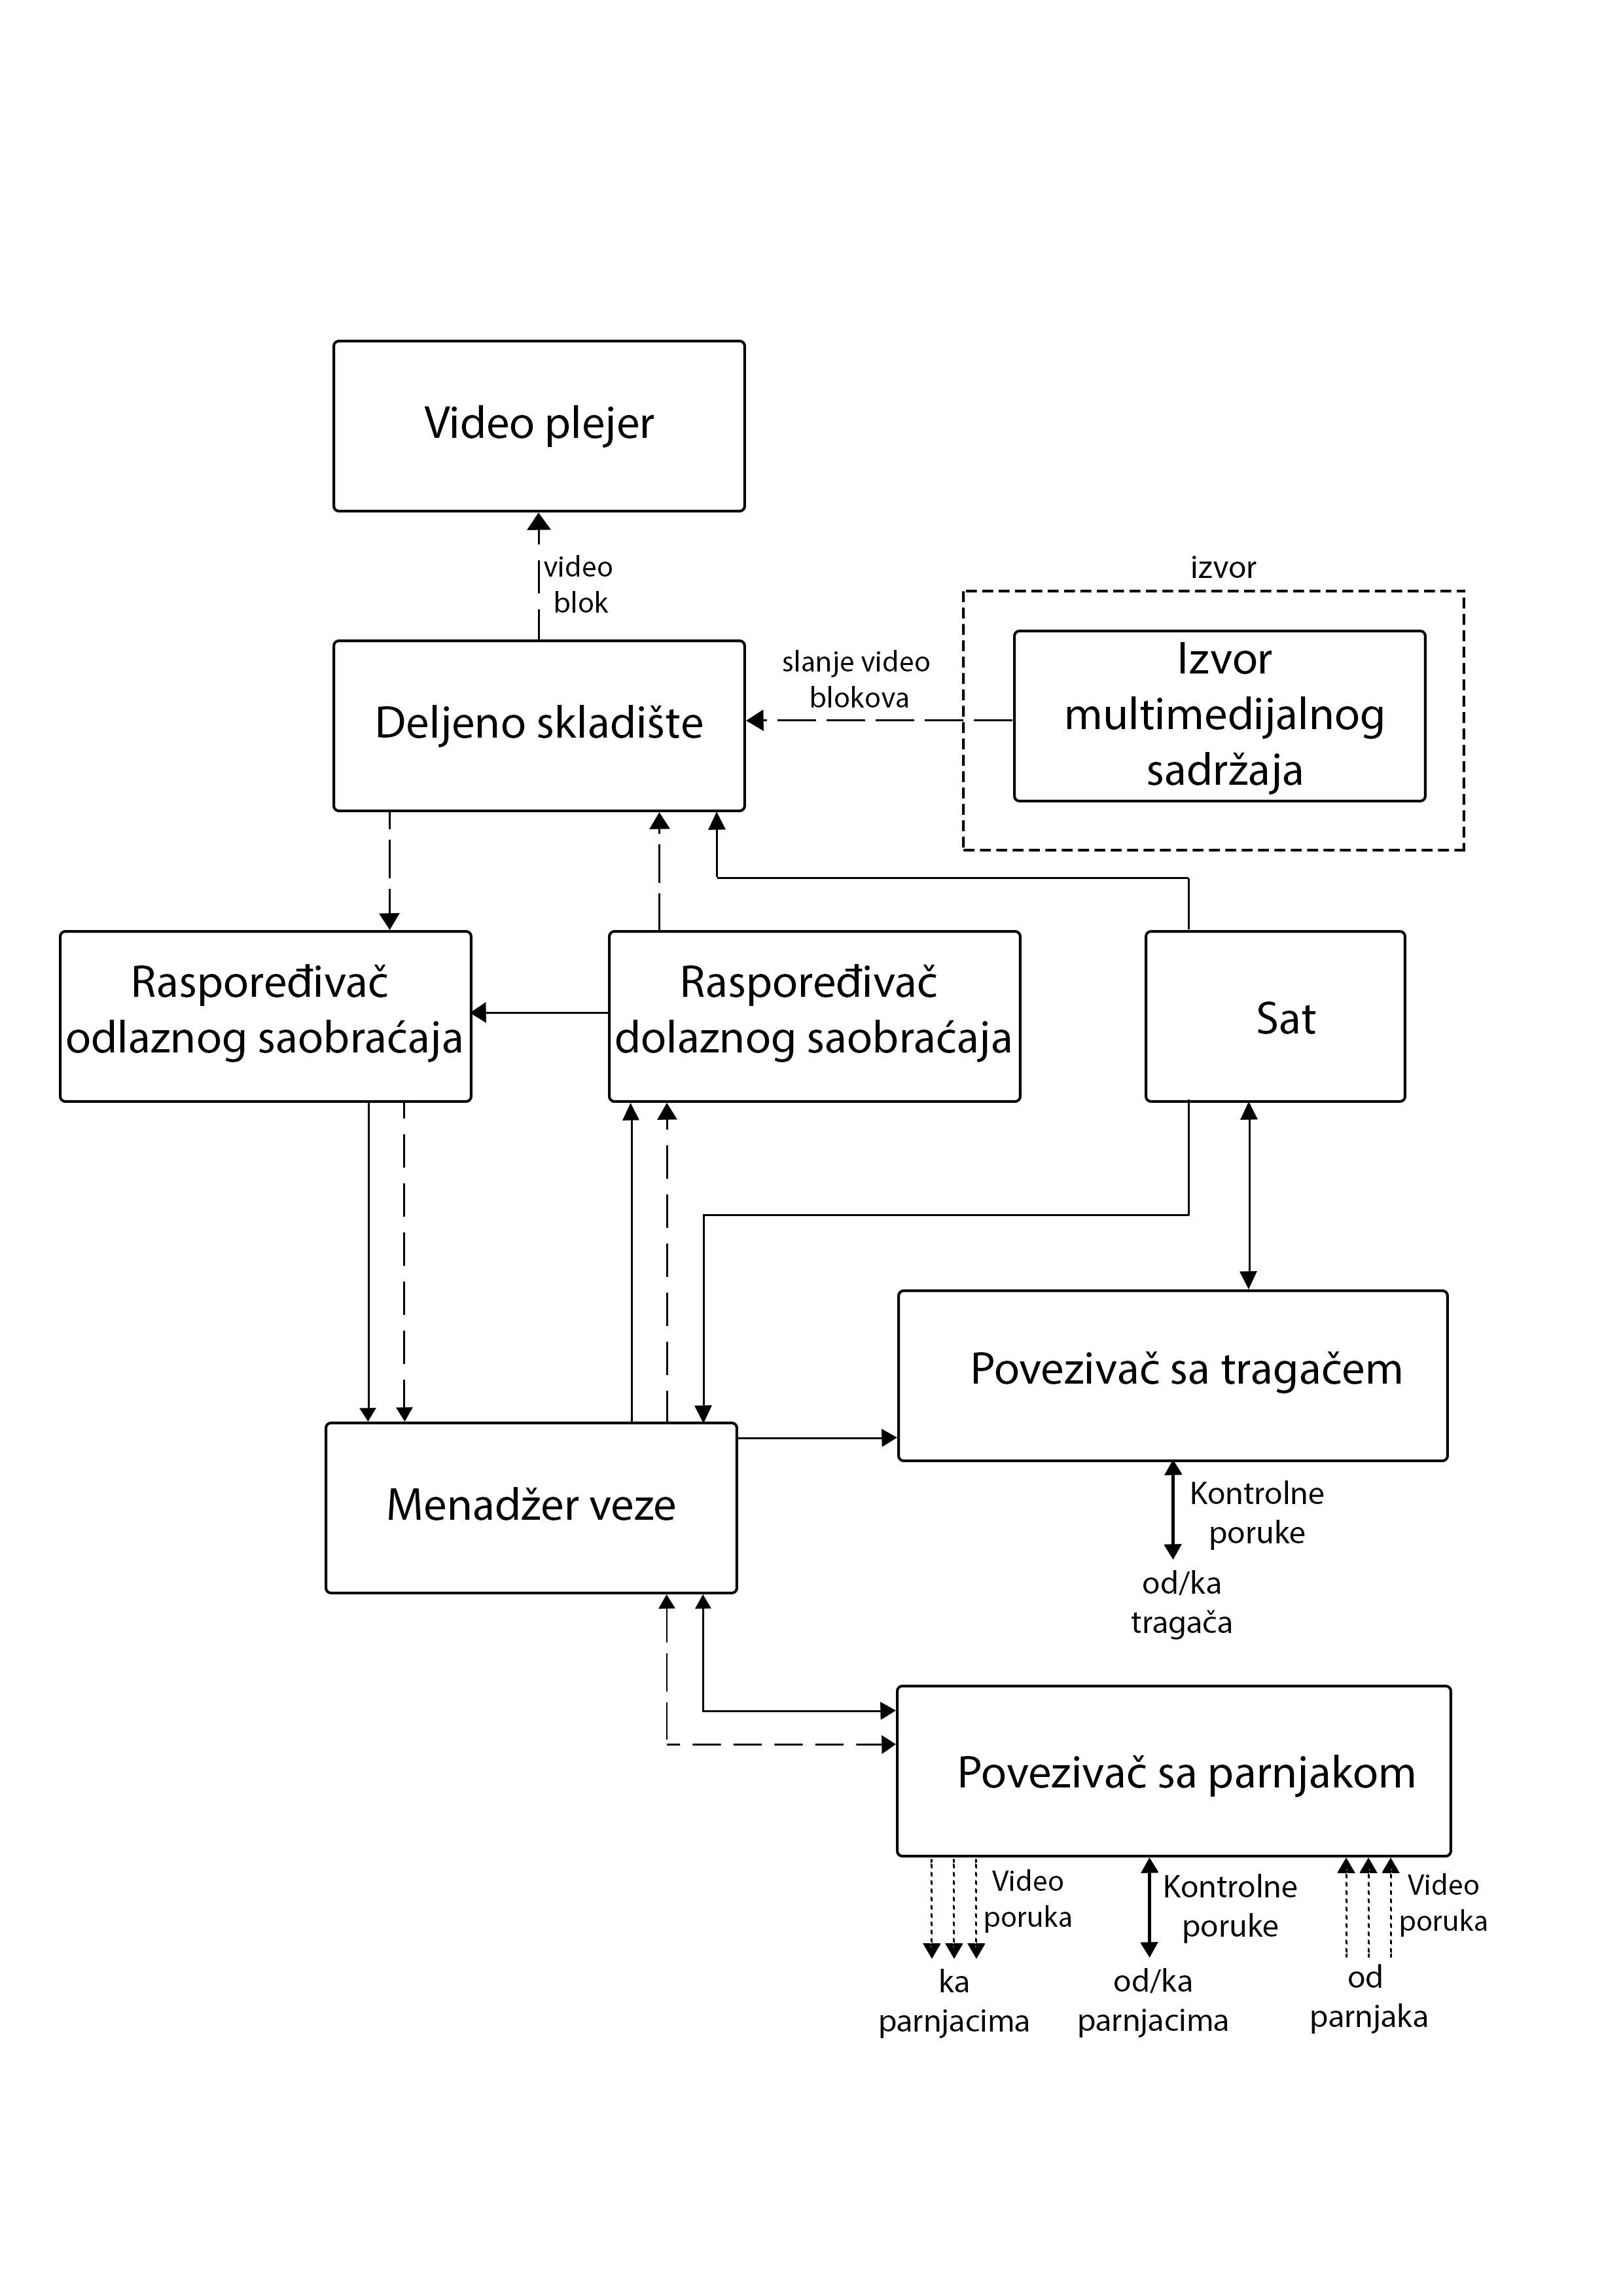
\includegraphics[width=0.85\textwidth]{slike/arhitektura-sistema.png}
  \caption{Arhitektura parnjaka. Isprekidane linije označavaju video podatke, pune linije označavaju kontrolne poruke.}
  \label{fig:arhitektura}
\end{figure}
\par

Kako je Kikkar složen sistem bilo je neophodno izvršiti prepoznavanje odgovarajućih celina i razdvajanje sistema na delove. Pojednostavljen model softverske arhitekture parnjaka prikazan je na slici \ref{fig:arhitektura}. Identičan model koristi i parnjak i izvor. Jedina razlika koja razdvaja parnjaka od izvora u modelu je ta što izvor sadrži dodatnu komponentu - izvor multimedijalnog sadržaja. Ova komponenta omogućava izvoru da uzima multimedijalni sadržaj koji je potrebno distribuirati kroz mrežu. Sadržaj može biti unapred pripremljen ili trenutno emitovan. U nastavku sledi opis svakog dela modela, njegovog zaduženja i opis podataka koje sadrži.


\subsubsection{Povezivač sa tragačem}
\label{implementacija.2.3.1}

Komponenta \textit{povezivač sa tragačem} (u programu klasa \texttt{ServerConnector}) predstavlja modul koji se koristi za komunikaciju parnjaka i tragača. Komunikacija se odvija uz pomoć HTTP i NTP protokola. Komponenta od podataka čuva informacije o željenom kanalu i datum poslednje izmene podataka. Informacije o željenom kanalu koriste se za prosleđivanje tačnog upita o određenom kanalu tragača. Informacija o poslednjoj modifikaciji služi za smanjenje opterećenja tragača. Ukoliko se jato nije promenilo od poslednje modifikacije, tragač ignoriše zahtev za novim parnjacima. 

Funkcionalnosti koje ova klasa obezbeđuje su učitavanje JSON fajla koji sadrži podatke o kanalu u okviru metode \texttt{loadJson(String json)}. JSON fajl obezbeđuje tragač prilikom registrovanja kanala. Kako se većini metoda tragača pristupa GET zahtevima neophodno je kreirati URL upite. Metod koji se koristi za tu svrhu je \texttt{createURL(String baseURL, Map<String, String> parameters)}, gde \textit{baseURL} predstavlja url na koji želimo da kreiramo upit. Mapa parametara predstavlja parametre koje želimo da dodamo upitu. Kreiranje zaglavlja HTTP poruke se izvršava u metodi \texttt{getURLConnection(URL url)}, gde je \textit{url} konkretan url za koji se kreira upit. Za inicijalnu konekciju sa tragačem koristi se metoda \texttt{connectToServer(URL url)}. Za sinhronizaciju vremena sa serverom koristi se metod \texttt{synchronizeTime(NTPUDPClient client, String ntpServer)}. Argument \textit{client} predstavlja klijentsku implementaciju NTP protokola, a argument \textit{ntpServer} predstavlja adresu NTP servera. U okviru klasnih metoda pristupa se klasi \textit{Sat} o kojoj će biti više reči u poglavlju \ref{implementacija.2.3.4}. U samom protokolu tragač obezbeđuje tačno vreme, ali se ovde zbog jednostavnosti koriste javno dostupni NTP serveri. Bitno je primetiti da se na ovaj način ne umanjuje opštost protokola. Lista parnjaka dobija se pozivanjem metoda \texttt{getPeerInfoList(URL url)} dok se obaveštavanje tragača o aktivnosti vrši se metodom \texttt{sendStayAliveMessage(URL url)}. Prilikom napuštanja kanala iz bilo kog razloga koristi se metod \texttt{sendLeaveMessage(URL url)}.  


\subsubsection{Povezivač sa parnjakom}
\label{implementacija.2.3.2}

Komponenta \textit{povezivač sa parnjakom} (u programu klasa \texttt{PeerConnector}) predstavlja modul koji se koristi za komunikaciju parnjaka sa ostatkom jata. Komunikacija se odvija uz pomoću UDP protokola. Ova komponenta je najniža komponenta za komunikaciju sa parnjacima i kao takva ne donosi nikakve odluke već samo izvršava naredbe viših komponenti. Modul čuva sve pakete koje je parnjak dobio preko mreže u blokirajućem redu kao i podatke o samom sebi.

Komponenta sadrži veliki broj metoda. Većina ovih metoda se ipak ne koristi direktno. U ovom radu opisaćemo samo metode koje bi prosečni korisnik klase želeo da koristi. Za razumevanje ostalih metoda dovoljno je razumeti protokol opisan u poglavlju \ref{chp:p2p-protokol}. 

Za slanje paketa neophodno je pozivanje metoda \texttt{void send(DatagramPacket sendDataPacket, DatagramSocket socket)}. Argumenti su paket \textit{sendDataPacket} koji želimo poslati i \textit{soket} preko koga želimo izvršiti slanje. Za primanje podataka sa mreže koristi se metod \texttt{void startRecievePacketLoop(DatagramSocket socket)}. U okviru ovog metoda puni se blokirajuć red.

Prvi zadatak parnjaka kod pristupanja jatu je razmena ping-pong poruke. Ping poruka se šalje metodom \texttt{void sendPingMessages(List<PeerInformation> \\ neighbourPeers, ConnectionType connectionType, DatagramSocket socket, \\Short  clubNum)}. Lista parnjaka \textit{neighbourPeers} predstavlja listu potencijalnih komšija, \textit{connectionType} predstavlja tip konekcije opisane u poglavlju \ref{implementacija.2.2}, \textit{socket} predstavlja apstrakciju soketa preko koga se vrši saobraćaj a \textit{clubNum} broj kluba kome parnjak pripada. U okviru ove metode svakom od parnjaka iz potencijalne liste komšija šalje se ping poruka i postavlja se novo stanje parnjaka na čekanje pong poruke. Pong poruka se šalje metodom \texttt{void sendPongMessage(List<PeerInformation> neighbourPeers, PeerInformation peer, PingMessage pingMessage, \\DatagramSocket socket)}. Lista parnjaka \textit{neighbourPeers} predstavlja listu već postojećih komšija, \textit{peer} predstavlja parnjaka kome se odgovara na ping poruku \textit{pingMessage} dok \textit{socket} predstavlja apstrakciju soketa preko koga se vrši saobraćaj. U okviru ove metode proverava se koliko veza i uskladištenih podataka ima parnjak i šalje pong poruka. 

Nakon što su razmenjene ping-pong poruke šalju se request-response poruke. Request poruka se šalje metodom \texttt{void sendRequestMessage(List<PeerInformation> neighbourPeers, DatagramSocket socket, ConnectionType connectionType)}. Argument \textit{neighbourPeers} odgovara listi parnjaka sa kojima želimo da se povežemo, \textit{socket} je apstrakcija soketa a \textit{connectionType} tip konekcije koju želimo da uspostavimo. U okviru ove metode svakom parnjaku iz liste se šalje request poruka i postavlja stanje na čekanje response poruke. Response poruka se šalje metodom \texttt{void sendResponseMessage(PeerInformation peer, PacketWrapper packet, \\ DatagramSocket socket)}, gde \textit{peer} predstavlja parnjaka kome se šalje \textit{packet} preko \textit{socket}-a. Nakon što je response poruka poslata postavlja se status parnjaka na povezano.

Za slanje keep-alive poruke parnjaku opisane u poglavlju \ref{Kikkar.4} koristi se metod \texttt{void sendKeepAliveMessage(PeerInformation peer, DatagramSocket socket)}. Argument \textit{peer} odgovara parnjaku kojem se šalje poruka dok \textit{socket} predstavlja apstrakciju soketa preko koga se odvija saobraćaj.
			

\subsubsection{Menadžer veze}
\label{implementacija.2.3.3}

Komponenta \textit{menadžer veze} (u programu klasa \texttt{ConnectionManager}) predstavlja modul koji se koristi za održavanje topologije parnjaka. Glavni zadatak ove komponente je da sakrije topologiju mreže od viših nivoa aplikacije i da koordiniše komunikaciju između tragača i parnjaka. U zavisnosti da li je aplikacija pokrenuta u režimu izvora ili parnjaka, menadžer veze istim metodama različito održava topologiju i procesira pakete u skladu sa protokolom. Modul od podataka čuva reference ka povezivaču sa tragačem i parnjakom, soket, podatke o trenutnom kanalu, listu svih parnjaka, listu svih dobijenih pong poruka, sat, pakete za viši nivo aplikacije u blokirajućem redu kao i pristupni token tragača.

Za učitavanje JSON fajla koristi se metod \texttt{void loadJson(String rawJson)}. Ovaj metod samo prosleđuje parametre istom metodu povezivača sa tragačem. Da bi se pokrenulo osluškivanje i procesiranje paketa koristi se metod \texttt{void start()}. U okviru ovog metoda pokreće se u zasebnoj niti metod za primanje podatka klase povezivač sa parnjakom. Takođe, u okviru nje se radi kontrola zagušenja i eventualno slanje keep-alive poruke komšijama \ref{Kikkar.4}, kao i provera i održavanje topologije \ref{Kikkar.2}. Za svaki primljeni paket proverava se da li je u dobrom redosledu i prosleđuje metodu za obradu paketa. U okviru ove metode svi paketi koji ne predstavljaju video sadržaj već kontrolne poruke se obrađuju u skladu sa protokolom. 

Kako bismo poslali pakete svim komšijama koristimo metod \texttt{void sendAll(\\PacketWrapper.Builder wrap, List<String> uninterestedPeerIp, \\PeerStatus peerStatus)}. Argument \textit{wrap} predstavlja poruku koja se šalje, lista \textit{uninterestedPeerIp} predstavlja listu komšija koji nisu zainteresovani za poruku dok \textit{peerStatus} predstavlja status komšija kojima se šalje poruka. Svim komšijama koji imaju odgovarajući status i ne nalaze se na listi nezainteresovanih biće isporučena poruka. Najpre se poruka isporučuje komšijama u klubu pa tek onda ostalima da bi se što brže distribuirala. Ukoliko poruku želimo da pošaljemo jednom parnjaku koristi se metod \texttt{void sendOne(PacketWrapper.Builder wrap, String IpAddress)} gde \textit{wrap} predstavlja poruku a \textit{IpAddress} adresu parnjaka kome se poruka šalje. Ukoliko želimo da pošaljemo poruku svim komšijama u klubu koristimo metod \texttt{void sendToClub(PacketWrapper.Builder wrap, PeerStatus peerStatus, int \\clubNum)}. Kao i u prethodnim metodama argument \textit{wrap} predstavlja poruku koja se šalje, \textit{peerStatus} predstavlja status komšija kojima se šalje poruka a \textit{clubNum} broj kluba.


\subsubsection{Sat}
\label{implementacija.2.3.4}

Komponenta \textit{sat} (u programu klasa \texttt{ClockSingleton}) predstavlja modul koji se koristi za ujednačavanje vremena svih parnjaka u mreži. Sat koristi unikat (eng. \textit{singleton}) uzorak za projektovanje. Pri razvoju aplikacija često je potrebno omogućiti korišćenje samo jedne instance određene klase iz konceptualnih ili arhitekturalnih razloga. Treba biti oprezan pri korišćenju unikata jer sa njim uvodimo globalno stanje u aplikaciju čime se povećava njena kompleksnost. U većini slučajeva ubrizgavanje zavisnosti (eng. \textit{dependency injection}) treba koristiti umesto unikata. Korišćenjem ubrizgavanja zavisnosti ne postoji direktna zavisnost između klasa aplikacije jer objekat ne zna koja je klasa u pitanju već zna samo njen javni interfejs. Međutim, u aplikaciji se klasa sat koristi u različitim delovima programa te bi korišćenje ubrizgavanja zavisnosti previše zakomplikovalo kreiranje objekata željenih klasa pa se iz tog razloga koristi unikat.

Formiranje i dobijanje unikat objekta ostvaruje se korišćenjem metode \\\texttt{ClockSingleton getInstance()}. 
Takođe treba obratiti pažnju i na to da je konstruktor deklarisan sa privatnim pravima pristupa. Klasa koristi vremensku zonu Europe/Belgrade. Da bismo dobili vreme koje je isto svuda u mreži koristimo metod \texttt{Long getcurrentTimeMilliseconds()}.


\subsubsection{Raspoređivač dolaznog saobraćaja}
\label{implementacija.2.3.5}

Komponenta \textit{raspoređivač dolaznog saobraćaja} (u programu implementirana klasom \texttt{DownloadScheduler}) predstavlja modul koji se koristi za menadžerisanje video sadržaja i kontrolnih poruka koje su povezane sa video sadržajem. Podaci koje klasa čuva su deljeno skladište za video sadržaj, menadžer veze za komunikaciju sa mrežom, raspoređivač odlaznog saobraćaja kojem se prosleđuju potrebne akcije za slanje video sadržaja i video kontrolnih poruka kroz mrežu. Razlikuju se metodi za procesiranje paketa u zavisnosti da li je aplikacija pokrenuta u modu parnjaka ili izvora.

Da bi se pokrenulo preuzimanje odgovarajućih paketa od menadžera veze koristi se metod \texttt{void startDownload()}. Za obradu paketa u skladu sa opisanim protokolom koristi se metod \texttt{void processPacket(Pair<String,PacketWrapper> packetPair)}. U okviru ove metode poziva se i raspoređivač odlaznog saobraćaja ukoliko za to postoji potreba.


\subsubsection{Raspoređivač odlaznog saobraćaja}
\label{implementacija.2.3.6}

Komponenta \textit{raspoređivač odlaznog saobraćaja} (u programu implementirana klasom \texttt{DownloadScheduler}) predstavlja modul koji se koristi za menadžerisanje slanja video sadržaja i kontrolnih poruka koje imaju veze sa video sadržajem. Podaci koje klasa čuva su deljeno skladište za preuzimanje video sadržaja, menadžer veze za komunikaciju sa mrežom za dalje prosleđivanje poruka. Razlikuju se metodi za procesiranje paketa u zavisnosti da li je aplikacija pokrenuta u modu parnjaka ili izvora.

Za slanje kontrolne poruke, opisane u poglavlju \ref{Kikkar.5} koristi se metod \texttt{void \\ sendControlMessage(ControlMessage message)}. Za slanje nezainteresovane poruke, opisane u poglavlju \ref{Kikkar.3},  koristi se metod \texttt{void sendNotInterested(Pair<String, PacketWrapper> haveMessagePair)}. Za slanje video snimka koristi se metod \texttt{void sendVideo(int currentVideoNum, \\List<String> currentVideoNotInterestedIpAddresses)}, gde \textit{currentVideoNum} odgovara jedinstvenom broju video snimka koji je potrebno poslati dok \textit{currentVideoNotInterestedIpAddresses} IP adresama parnjaka koji nisu zainteresovani za sadržaj. Za odgovor na traženje video snimka koristi se metod \texttt{void sendVideo(void sendResponseMessage(Pair<String, PacketWrapper> packetPair, int[]\\ videoNum)}. Za pronalaženje nedostajajućih video snimaka koristi se metod \texttt{void getMissingVideoNum()}.


\subsubsection{Deljeno skladište}
\label{implementacija.2.3.7}

Komponenta \textit{deljeno skladište} (u programu klasa \texttt{SharingBufferSingleton}) predstavlja modul koji se koristi za skladištenje multimedijalnog sadržaja i njegovo prosleđivanje video plejeru i sinhronizaciju video sadržaja. Koristi unikat obrazac za projektovanje na isti način i iz istog razloga kao i komponenta sat. Klasa čuva objekat klase sat, niz objekata video snimaka i objekat video plejer.

Pri korišćenju VLC plejera neophodno je zapisati podatak iz skladišta u fajl. Zapisivanje se ostvaruje metodom \texttt{void saveVideoPack(OutputStream os, int lastControlMessageVideoNum)}. U okviru ove metode osim snimanja sadržaja u fajl, briše se zastareli video sadržaj. Da bi se dobio broj trenutno uskladištenih podataka koristi se metod \texttt{int getNumberOfBufferedVideoContent()}. Za sinhronizaciju video sadržaja metodima opisanim u poglavlju \ref{Kikkar.5} koriste se metodi \texttt{void synchronizeVideoPlayTime(int currentVideoNum, ControlMessage controlMessage)} i \texttt{void synchronizeVideoPlayTime(int currentVideoNum)} gde je \textit{currentVideoNum} trenutni jedinstveni identifikator video sadržaja koji se prikazuje a \textit{controlMessage} kontrolna poruka koja se prikazuje. 


\subsubsection{Video plejer}
\label{implementacija.2.3.8}

Komponenta \textit{video plejer} (u programu klasa \texttt{VLCPlayer}) predstavlja modul koji se koristi za prikazivanje multimedijalnog sadržaja. Korsti se VLCj radni okvir za pokretanje instance nativnog VLC medijskog plejera i skrivanje kompleksnosti rada sa LibVLC. VLCj radi na Linux, Windows i MacOSX operativnim sistemima. Od podataka klasa sadrži instancu plejera i putanju do video sadržaja. 

Za prikazivanje video snimka koristi se metod \texttt{void playVideo()}. Dobijanje dužine trenutno prikazanog sadržaja vrši se metodom
\texttt{int getCurrentPlayTime()}.
 Da bi se izvršila sinhronizacija video plejera sa izvorom koristi se metod \texttt{void synchronizeVideo(int sourceVideoTime)} gde \textit{sourceVideoTime} predstavlja dužinu emitovanog snimka plejera.


\subsubsection{Izvor multimedijalnog sadržaja}
\label{implementacija.2.3.9}
Komponenta \textit{izvor multimedijalnog sadržaja} (u programu implementirana klasom \texttt{SourceVideoLoader}) predstavlja modul koji se koristi za prikupljanje multimedijalnog sadržaja. Multimedijalni sadržaj može biti snimljen ili emitovan. Ova komponenta se izdvaja od svih prethodno opisanih komponenti jer se povezuje sa ostalim komponentama samo u slučaju moda aplikacije izvor. Od podataka sadrži sat, deljeno skladište i raspoređivač odlaznog saobraćaja.

Učitavanje video sadržaja obezbeđeno je metodom \texttt{void loadVideo(String \\inputVideoPath, String outputVideoPath)} gde \textit{inputVideoPath} odgovara putanji na kojoj se nalazi video sadržaj a \textit{outputVideoPath} putanji na kojoj plejer očekuje video sadržaj. Vrši se učitavanje pojedinačnih blokova a zatim se čeka određeno vreme pre učitavanja sledećeg.
Potrebno vreme čekanja zavisi od karakteristika video snimka. Vreme čekanja se uvodi kako bi se sprečilo zagušenje izvora.
Za čitanje dela video bloka i njegovo slanje u jato koristi se metoda \texttt{void readChunk(InputStream is, int chunkNum)}.  Vreme čekanja zavisi od brzine kojom se blokovi šalju i broja blokova. Najpre se svaki blok snimi u deljeno skladište a zatim distribuira u mrežu.


%\pangrami

%\pangrami

% ------------------------------------------------------------------------------
\chapter{Zaključak}
% ------------------------------------------------------------------------------


% ------------------------------------------------------------------------------
% Literatura
% ------------------------------------------------------------------------------
\literatura

% ==============================================================================
% Završni deo teze i prilozi
\backmatter
% ==============================================================================

% ------------------------------------------------------------------------------

\end{document}
